% !TEX encoding = UTF-8 Unicode
\documentclass[11pt,a4paper]{article}
%\usepackage[T1]{fontenc}
%\usepackage[charter]{mathdesign}
\usepackage{graphicx}  \usepackage{mathptmx}
\usepackage{amsmath, amssymb}
\usepackage{gensymb}
%\usepackage{showkeys}
\usepackage{enumitem}
\usepackage{tikz}
\usepackage{tikz-cd}
\usepackage{wrapfig}
\usetikzlibrary{decorations.pathmorphing}
\tikzset{snake it/.style={decorate, decoration=snake}}
\usepackage{xpatch}
\topmargin = - 1.5 cm
\textheight = 24 cm
\textwidth = 16 cm
\oddsidemargin = -0.1 cm
\renewcommand{\theequation}{\thesection.\arabic{equation}}
\makeatletter
\@addtoreset{equation}{section}
\makeatother
%\usepackage{showkeys}
\newcommand{\third}{\mbox{\footnotesize $\frac{1}{3}$}}
\newcommand{\tthird}{\mbox{\footnotesize $\frac{2}{3}$}}
\newcommand{\quar}{\mbox{\footnotesize $\frac{1}{4}$}}
\newcommand{\half}{\mbox{\footnotesize $\frac{1}{2}$}}
\newcommand{\hi}[1]{\emph{\textbf{#1}}}
\newcommand{\qm}{quantum mechanics}
\newcommand{\er}{\eqref}
\renewcommand{\L}{\label} 
\newcommand{\beq}{\begin{equation}}
\newcommand{\eeq}{\end{equation}} 
\newcommand{\bea}{\begin{eqnarray}}
\newcommand{\eea}{\end{eqnarray}} \newcommand{\nn}{\nonumber}
\newcommand{\ol}{\overline}
\newcommand{\fwt}{{\sc fwt}}
\newcommand{\ovl}{\overline}
\newcommand{\ul}{\underline}
\newcommand{\wed}{\wedge}
 \newcommand{\til}{\tilde}
\newcommand{\raw}{\rightarrow} 
\newcommand{\rac}{\rightarrowtail}
\newcommand{\lac}{\leftarrowtail}
\newcommand{\law}{\leftarrow} \newcommand{\Raw}{\Rightarrow}
\newcommand{\hraw}{\hookrightarrow} \newcommand{\Law}{\Leftarrow}
\newcommand{\lraw}{\leftrightarrow}
\newcommand{\LRaw}{\Leftrightarrow}
\newcommand{\rlh}{\rightleftharpoons}
\newcommand{\ot}{\otimes} 
\newcommand{\la}{\langle} \newcommand{\ra}{\rangle}
\newcommand{\ran}{\mathrm{ran}}
\newcommand{\rst}{\upharpoonright} \newcommand{\cov}{\nabla}
\newcommand{\x}{\times}
\newcommand{\tps}{transition probability space}
\newcommand{\Lg}{Lie groupoid}
\newcommand{\tp}{transition probability}
\newcommand{\tpies}{transition probabilities} 
\newcommand{\clm}{classical mechanics}
\newcommand{\ca}{C*-algebra} \newcommand{\jba}{JB-algebra}
\newcommand{\jlba}{JLB-algebra} \newcommand{\rep}{representation}
\newcommand{\irrep}{irreducible representation}
\newcommand{\Hs}{Hilbert space} \newcommand{\Bs}{Banach space}
\newcommand{\BA}{Banach algebra} \newcommand{\mom}{momentum map}
\newcommand{\cin}{C^{\infty}} \newcommand{\cci}{C^{\infty}_c}
\newcommand{\sta}{$\mbox{}^*$-algebra}
\newcommand{\sthom}{$\mbox{}^*$-homomorphism}
\newcommand{\staut}{$\mbox{}^*$-automorphism}
\newcommand{\stiso}{$\mbox{}^*$-isomorphism}
\newcommand{\hv}{hidden variable}
\newcommand{\inp}[2]{\langle #1,#2 \rangle}
\newcommand{\MW}{Marsden--Weinstein} \newcommand{\HCM}{Hilbert
$C^*$-module} \newcommand{\vN}{von Neumann} \newcommand{\vna}{von
Neumann algebra}
\newcommand{\op}{^{\mbox{\tiny op}}}
\newcommand{\Exp}{\mathrm{Exp}}
\newcommand{\CA}{\mathcal{C}(A)} 
% Greek  
%
\newcommand{\al}{\alpha} \newcommand{\bt}{L\beta}
\newcommand{\gm}{\gamma} \newcommand{\Gm}{\Gamma}
\newcommand{\dl}{\delta} \newcommand{\Dl}{\Delta}
\newcommand{\ep}{\epsilon} \newcommand{\varep}{\varepsilon}
\newcommand{\zt}{\zeta} \newcommand{\et}{\eta}
 \newcommand{\vth}{\vartheta}
\newcommand{\io}{\iota} \newcommand{\kp}{\kappa}
\newcommand{\lm}{\lambda} \newcommand{\Lm}{\Lambda}
\newcommand{\rh}{\rho} \newcommand{\sg}{\sigma}
\newcommand{\Sg}{\Sigma} \newcommand{\ta}{\tau} \newcommand{\ph}{\phi}
\newcommand{\Ph}{\Phi} \newcommand{\phv}{\varphi}
\newcommand{\ch}{\ch} \newcommand{\ps}{\psi} \newcommand{\Ps}{\Psi}
\newcommand{\om}{\omega} \newcommand{\Om}{\Omega}
\newcommand{\ups}{\upsilon}
%
% German
%
\newcommand{\daw}{\!\downarrow}
\newcommand{\uaw}{\!\uparrow}
\newcommand{\kwm}{kwantummechanica}
\newcommand{\km}{klassieke mechanica}
\newcommand{\qh}{q_{\hbar}}
\newcommand{\Qh}{Q_{\hbar}}
\newcommand{\inv}{^{-1}}
\newcommand{\Tr}{\mbox{\rm Tr}\,} 
\newcommand{\A}{\mathfrak{A}} \newcommand{\B}{\mathfrak{B}}
\newcommand{\GC}{\mathfrak{C}} \newcommand{\GE}{\mathfrak{E}}
\newcommand{\GF}{\mathfrak{F}} \newcommand{\GG}{\mathfrak{G}}
\newcommand{\GI}{\mathfrak{I}} \newcommand{\K}{\mathbb{K}}
\newcommand{\GM}{\mathfrak{M}} \newcommand{\GN}{\mathfrak{N}}
\newcommand{\GU}{\mathfrak{U}} \newcommand{\GW}{\mathfrak{W}}
\newcommand{\GS}{\mathfrak{S}} \newcommand{\g}{\mathfrak{g}}
\newcommand{\GQ}{\mathfrak{Q}}
\newcommand{\h}{\mathfrak{h}} 
\newcommand{\m}{\mathfrak{m}} \newcommand{\Gl}{\mathfrak{l}}
\newcommand{\GP}{\mathfrak{P}} \newcommand{\s}{\mathfrak{s}}
\renewcommand{\t}{\mathfrak{t}}
%
% Calligraphic
%
%\newcommand{\CA}{{\mathcal A}} 
\newcommand{\CB}{{\mathcal B}}
\newcommand{\CC}{{\mathcal C}} \newcommand{\CF}{{\mathcal F}}
%\newcommand{\CD}{{\mathcal D}} 
\newcommand{\CE}{{\mathcal E}}
\newcommand{\CG}{{\mathcal G}} \renewcommand{\H}{{\mathcal H}}
\newcommand{\CJ}{{\mathcal J}} \newcommand{\CI}{{\mathcal I}}
\newcommand{\CK}{{\mathcal K}}   \newcommand{\CL}{{\mathcal L}}   
 \newcommand{\CM}{{\mathcal M}}
\newcommand{\CN}{{\mathcal N}} \newcommand{\CS}{{\mathcal S}}
\newcommand{\CO}{{\mathcal O}} \newcommand{\CP}{{\mathcal P}}
\newcommand{\CQ}{{\mathcal Q}} \newcommand{\CR}{{\mathcal R}}
\newcommand{\CT}{{\mathcal T}} \newcommand{\CV}{{\mathcal V}}
\newcommand{\CW}{{\mathcal W}} \renewcommand{\P}{{\mathcal P}}
\renewcommand{\L}{\label}
\newcommand{\CZ}{{\mathcal Z}}
%
% blackboard
%
\newcommand{\C}{{\mathbb C}} 
\newcommand{\N}{{\mathbb N}} \newcommand{\R}{{\mathbb R}}
\newcommand{\T}{{\mathbb T}} \newcommand{\Z}{{\mathbb Z}}
%
% sans serif
%
\newcommand{\SSB}{\mathsf{B}} \newcommand{\SG}{\mathsf{G}}
\newcommand{\SSH}{\mathsf{H}} \newcommand{\SU}{\mathsf{U}}
\newcommand{\SSP}{\mathsf{P}} \newcommand{\SSp}{\mathsf{p}}
\newcommand{\SSV}{\mathsf{V}} \newcommand{\SM}{\mathsf{M}}
\newcommand{\SSS}{\mathsf{S}} %
% bold
%
\newcommand{\bofe}{\mathbf{e}} \newcommand{\bofu}{\mathbf{u}}
\newcommand{\bofp}{\mathbf{p}} \newcommand{\bfp}{\mathbf{p}}
\newcommand{\bfe}{\mathbf{e}} \newcommand{\bfu}{\mathbf{u}}
\newcommand{\bg}{\mathbf{g}} \newcommand{\bR}{\mathbf{R}}
\newcommand{\ba}{\mathbf{a}}\newcommand{\bb}{\mathbf{b}}
\newcommand{\fb}{\mathbf{u}}
 \newcommand{\bF}{\mathbf{F}} \makeatletter
 \newcommand{\enp}{\hfill\mbox{}\qed}
\makeatletter
\def\moverlay{\mathpalette\mov@rlay}
\def\mov@rlay#1#2{\leavevmode\vtop{%
   \baselineskip\z@skip \lineskiplimit-\maxdimen
   \ialign{\hfil$\m@th#1##$\hfil\cr#2\crcr}}}
\newcommand{\charfusion}[3][\mathord]{
    #1{\ifx#1\mathop\vphantom{#2}\fi
        \mathpalette\mov@rlay{#2\cr#3}
      }
    \ifx#1\mathop\expandafter\displaylimits\fi}
\makeatother

\newcommand{\cupdot}{\charfusion[\mathbin]{\cup}{\cdot}}
\newcommand{\Dom}{\ensuremath{\mathrm{Dom}}}
\newcommand{\slim}{\ensuremath{\mathop{\text{s-lim}}}}
\renewcommand{\cov}{\covered}
\newcommand{\bigcupdot}{\charfusion[\mathop]{\bigcup}{\cdot}}
\newcommand{\mghd}{\textsc{mghd}}
\newcommand{\pde}{\textsc{pde}}
\newcommand{\pp}{\mathfrak{p}}
\newcommand{\Ad}{\mathrm{Ad}}
\newcommand{\ad}{\mathrm{ad}}
\newcommand{\Co}{\mathrm{Co}}
\newcommand{\iso}{\mathrm{Iso}}
\newcommand{\M}{\tilde{M}}
\renewcommand{\g}{\tilde{g}}
\newcommand{\tn}{\tilde{\nabla}}
\newcommand{\ali}{\begin{align}}
\newcommand{\elin}{\end{align}}
\newcommand{\X}{\mathfrak{X}}
\newcommand{\gnc}{{\sc gnc}}
\newcommand{\n}{\nabla}
\newcommand{\XM}{\mathfrak{X}(M)}
\newcommand{\p}{\partial}
\newcommand{\CD}{\mathcal{D}}
\renewcommand{\k}{\tilde{k}}
\renewcommand{\g}{\tilde{g}}
\renewcommand{\gg}{\mathfrak{g}}
\newcommand{\kk}{\mathfrak{h}}
\newcommand{\GR}{{\sc gr}}
\newcommand{\Ric}{\mathrm{Ric}}
\newcommand{\Riem}{\mathrm{Riem}}
\newtheorem{theorem}{Theorem}[section]
\newtheorem{lemma}[theorem]{Lemma}
\newtheorem{proposition}[theorem]{Proposition}
\newtheorem{corollary}[theorem]{Corollary}
\newtheorem{definition}[theorem]{Definition}
\newtheorem{example}[theorem]{Example}
\newenvironment{proof}[1][Proof]%
{ \begin{trivlist}%
  \item[\hskip \labelsep {\bfseries #1}]%
}%
{ \end{trivlist}%
}
\newcommand{\qed}{\nobreak\hfill$\Box$}
\newcommand{\qedhere}{\tag*{$\Box$}}
\begin{document}
\pagenumbering{arabic} \setlength{\unitlength}{1cm}\cleardoublepage
\date\nodate
\begin{center}
\begin{LARGE}
{\bf Singularities, black holes, and cosmic censorship: \smallskip

A tribute to Roger Penrose}\end{LARGE}
\bigskip

\begin{Large}
 Klaas Landsman
 \end{Large}
 \medskip
 
 \begin{large}
%Institute for Mathematics, Astrophysics, and  Particle Physics (IMAPP),
  Department of Mathematics, Radboud University, Nijmegen, The Netherlands\\
Email:
\texttt{landsman@math.ru.nl}
\end{large}
\smallskip
 \begin{abstract} 
\noindent 
In the light of his recent (and fully deserved) Nobel Prize, this pedagogical paper draws attention to a fundamental tension that drove Penrose's work on general relativity. His 1965 singularity theorem (for which he got the prize) does not in fact imply the existence of black holes (even if its assumptions are met). Similarly, his versatile definition of a singular space-time does not match the generally accepted definition of a black hole (derived from his concept of null infinity). To overcome this, Penrose launched his cosmic censorship conjecture(s), whose evolution we discuss. In particular, we review both his own (mature) formulation and its later, inequivalent reformulation in the \pde\ literature. As a compromise, one might say that  in ``generic'' or ``physically reasonable'' space-times, weak cosmic censorship postulates the \emph{appearance and stability of event horizons}, whereas  strong cosmic censorship asks for the \emph{instability and ensuing disappearance of Cauchy horizons}.
As an \emph{encore}, an appendix by Erik Curiel  reviews the early history of the \emph{definition} of a black hole.
\end{abstract}\end{center}
\tableofcontents

 \begin{center}
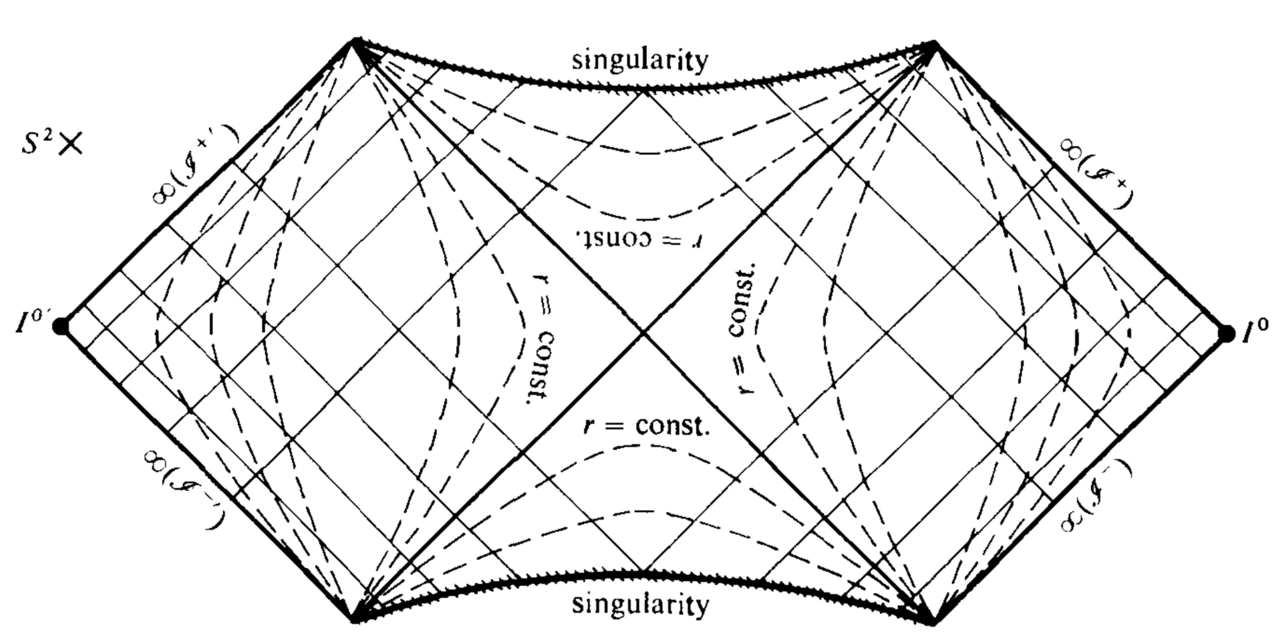
\includegraphics[width=0.5\textwidth]{PD1968.png} 
\end{center}
\emph{Conformal diagram (Penrose 1968, p.\ 208, Fig.\ 37): `The Kruskal picture with conformal infinity represented.'
Penrose usually drew his own figures in a  professional, yet playful and characteristic way. }


\thispagestyle{empty}
\renewcommand{\thefootnote}{\arabic{footnote}}
\newpage \setcounter{footnote}{0}
\section{Historical introduction}\label{HI}
Roger Penrose got half of the 2020 Physics Nobel Prize ``for the discovery that black hole formation is a robust prediction of the general theory of relativity''. This prize was well deserved, since, jointly with Hawking and others, Penrose  has shaped our (mathematical) thinking about general relativity (\GR) and black holes since the 1960s--70s. He would also deserve the Abel Prize for this,  shared with Yvonne Choquet-Bruhat: their combination would  highlight the fact that two originally distinct traditions in the history of mathematical \GR\ have now converged. In the wake of the work of Einstein (1915), these traditions may be said to have originated with Hilbert (1917) and Weyl (1918ab), respectively, as follows. 

 It would be fair to say that Hilbert mainly looked at \GR\ from the point of view of \pde s,\footnote{See 
   Stachel (1992) for an analysis of Hilbert's contribution, as well as for the history of the Cauchy problem of \GR\ up to Choquet-Bruhat, whose contributions were reviewed by  Ringstr\"{o}m (2015) as well as by herself 
    (Choquet-Bruhat, 2014, 2018).} whereas Weyl--once Hilbert's PhD student in functional analysis--had a more geometric view, combined with an emphasis on causal structure.  These different perspectives initially developed  separately, in that the causal theory did not rely on the \pde\ theory whilst for a long time the  \pde\ results were  local in nature.  Penrose contributed decisively to the causal approach to \GR, with its
 characteristic emphasis on the \emph{conformal structure},\footnote{Inspired by special rather than general relativity,  Robb (1914, 1936), Reichenbach (1924),  Zeeman (1964), and  others axiomatized causal structure as a specific \emph{partial order}, as Penrose knew well. } i.e.\ the equivalence class of the metric tensor $g$ under a rescaling $g_{\mu\nu}(x)\mapsto e^{\lm(x)} g_{\mu\nu}(x)$, 
  with $\lm$ an arbitrary smooth function of space and time. Though Weyl (1918b), p.\ 397,  mentions the analogy with Riemann surfaces,\footnote{Riemann surfaces  may equivalently be defined as either one-dimensional complex manifolds or as  two-dimensional Riemannian manifolds \emph{up to conformal equivalence}. 
 Modestly, Weyl does not cite his own decisive contribution to their theory (Weyl, 1913).  This equivalence undoubtedly also influenced Penrose's work on \GR\  and its derivatives like twistor theory. } his real argument for conformal invariance was  that what he calls \emph{Reine Infinitesimalgeometrie} must go beyond Riemannian geometry, which (so he thinks) suffers from the inconsistency that parallel transport of vectors (through the metric or Levi-Civita connection, a concept Weyl himself had co-invented) preserves their length. This makes length of vectors an absolute quantity, which a  `pure infinitesimal geometry' or a theory of \emph{general} relativity should not tolerate. To remedy this, Weyl introduced the idea of \emph{gauge invariance},  in that the laws of nature should be invariant under the above rescaling. To this end, he introduced what we now call a gauge field $\phv=\phv_{\mu}dx^{\mu}$ and
 a compensating transformation $\phv_{\mu}(x)\mapsto  \phv_{\mu}(x)-\p_{\mu} \lm(x)$, and identified $\phv$ with the electromagnetic potential (i.e.\ $A$). Dancing to the music of time, he then proposed that the pair $(g,\phv)$ describes all of physics. The idea of gauge symmetry has lasted and forms one of the keys to modern high-energy physics and quantum field theory: 
   though misplaced in the \emph{classical gravitational} context in which he proposed it,\footnote{See Einstein's negative reaction to Weyl (1918b) in Einstein (2002), Doc.\ 8. See also Goenner (2004), \S 4.1.3. }  through the Standard Model it has ironically become a cornerstone of \emph{non-gravitational quantum} physics! 

The conformal structure of a Lorentzian manifold determines the light cones, and as such
 Weyl was not the only author to discuss causal structure. For example, Einstein (1918) himself wondered if gravitational waves propagate with the speed of light, and showed this in a linear approximation; Weyl mentions this also.\footnote{See e.g.\ page 251 of the English translation of the fourth edition of  \emph{Raum - Zeit - Materie} (Weyl, 1922).} 
The themes of gravitational radiation, conformal invariance,  and causal order were combined and came to a head in the work of Penrose,\footnote{This intriguing history largely remains to be written. For the moment, see e.g.\ Thorne (1994), Frauendiener  (2000), Friedrich (2011),  Wright (2013, 2014), Ellis (2014), as well as \emph{Oral History Interviews: Roger Penrose} (1989) by Alan Lightman, \texttt{https://www.aip.org/history-programs/niels-bohr-library/oral-histories/34322}. Finally,
\emph{Extra Time: Professor Sir Roger Penrose in conversation with Andrew Hodges} (2014), available on YouTube, is a great and intimate portrait.
 } who also received additional inspiration from the Dutch artist M.C. Escher and the spinor theory of Dirac.
 In Penrose (1963, 1964, 1965, 1966, 1968, 1972) he introduced most of the global causal techniques and topological ideas   that are now central to any serious mathematical analysis of both \GR\ and Lorentzian geometry (O'Neill, 1983; Minguzzi, 2019). An important exception is global hyperbolicity, which has its roots in the work of Leray (1953) and was adapted to \GR\ by Choquet-Bruhat (1967) and Geroch (1970). Global hyperbolicity is the main concept through which the causal theory meets the \pde\ theory, but Penrose  hardly worked on the \pde\ side. 

The second piece of history one needs in order to understand Penrose's  contributions that are relevant to his Nobel Prize, is astrophysical. Briefly:\footnote{See  Israel (1987), Luminet (1992), Thorne (1994),  Melia (2009),  Sanders (2014), 
Curiel (2019a), and Falcke (2020)  for history, 
and Misner, Thorne, \& Wheeler (1973), Joshi (1993, 2007),   Poisson (2004), and  Weinberg (2020) for theory.} relatively light stars retire as white dwarfs, in which nuclear burning has ended and inward gravitational pressure is stopped by a degenerate electron gas. In 1931 Chandrasekhar  discovered that this works only for masses $m\leq 1.46 M_{\odot}$, where $M_{\odot}$ is the solar mass. Heavier stars collapse into neutron stars (typically after a supernova explosion), but also these have an upper bound on their mass, as first suggested by Oppenheimer \& Volkoff (1939); the current value is about $2.3  M_{\odot}$.  Stars that are more massive cannot stop their gravitational collapse and unless they get rid of most of their mass/energy they collapse completely.\footnote{Note that supermassive black holes like Sagittarius A* and M87* are formed by (secondary) accretion rather than collapse.}
 But what  does this mean mathematically?

%The current view is that sufficiently heavy stars (or other configurations of massive objects) collapse into
% a black hole, which in turn begs the question what \emph{that} means.
 Most of the early intuition came from the Schwarzschild solution, seen as a  model of the final state of such a collapse. This solution is spherically symmetric, and by Birkhoff's theorem any such vacuum solution must be Schwarzschild (or Minkowski). It has
 two very notable features, namely \emph{a curvature singularity as $r\raw 0$} and \emph{an event horizon at $r=2m$}.
Here it should be mentioned that  initially both  caused great confusion, even among the greatest scientists involved such as Einstein and Hilbert, though  Lema\^{i}tre was ahead of his time.\footnote{See Tipler, Clarke, Ellis (1980),  Godart (1992),
 Eisenstaedt (1993), Thorne (1994), Earman (1995, 1999),  and Earman \& Eisenstaedt (1999). Our understanding of the event horizon as a one-way membrane is usually attributed to Finkelstein (1958).}  Apart from their exact locations, these two features, then, may be taken to be the defining characteristics of a black hole, \emph{but especially the event horizon, which is held to be responsible for the ``blackness'' of the ``hole''.} 
 However, even short of a correct technical understanding of these features,
 from the 1920s until the 1950s most leading researchers in \GR\ (including Einstein, Eddington, as well as Landau's school in the Soviet Union, which covered all of theoretical physics) felt that at least the singularity was an artifact of the perfect spherical symmetry of the solution (and likewise for the big bang as described by the spherically symmetric Friedman/{\sc flrw} solution). This negative view also applied to the 
first  generally relativistic collapse model (Oppenheimer \& Snyder, 1939), now seen as groundbreaking, which is spherically  symmetric and therefore terminates in the Schwarzschild solution.

The achievement  usually attributed to Penrose (1965), culminating in his Nobel Prize, is that he 
settled (in the positive) the question whether a more general (i.e.\ non-spherically symmetric) collapse of sufficiently heavy stars (etc.) also leads to a black hole. But
if anyone understood this was \emph{not} the case for the construal of a black hole as an astrophysical object with event horizon,
  it was Penrose himself! He must have been the first to recognize that his singularity theorem from 1965 did not prove the existence of black holes; under suitable hypotheses (involving both the concentration of matter and the causal structure of space-time) it  proved merely the existence (but not even the precise nature or location) of incomplete null geodesics. As such, this implies neither the existence of a \emph{curvature} singularity (not even if the solution is close to Schwarzschild), nor that of an event horizon. 
   Leaving the former aside for the moment, the latter became the topic of what is now called  the  \emph{weak cosmic censorship conjecture}:\footnote{\label{PD} It is worth stressing that Penrose included a genericity restriction right from the beginning, \emph{pace}  Dafermos (2012), p.\ 55.
 The emphasis on initial data in the second formulation does not recur in the strong version of cosmic censorship below, but it is unavoidable in any form of weak cosmic censorship in order to exclude the naked big bang singularity from the conjecture: the point of the second (1979) formulation is that the singularity lies to the future of the Cauchy hypersurface in question. 
    }
  \begin{quote}
\begin{small}
We are thus presented with what is perhaps the most fundamental question of general-relativistic collapse theory, namely: does there exist a ``cosmic censor'' who forbids the appearance of naked singularities, clothing each one in an absolute event horizon? In one sense, a  ``cosmic censor'' can be shown \emph{not} to exist. For it follows from a theorem of Hawking that the ``big bang'' singularity is, in principle, observable. But it is not known whether singularities observable from outside will ever arise in a generic \emph{collapse} which starts off from a perfectly reasonable nonsingular initial state.  (Penrose, 1969,  p.\ 1162)

A system which evolves, according to classical general relativity with reasonable equations of state, from generic non-singular  initial data on a suitable Cauchy hypersurface, does not develop any spacetime singularity which is visible 
from infinity. (Penrose, 1979, p.\ 618)
\end{small}
\end{quote}
Following Penrose (1979) we give a precise mathematical version in \S\ref{Defs}, but in any case it should be clear that in order to prove the existence of black holes from suitable assumptions one needs \emph{both} Penrose's singularity theorem (which gives at least some kind of singularity) \emph{and} the weak cosmic censorship hypothesis (which gives the event horizon): the latter is the missing link between theorem and reality. 

Expanding the scope of cosmic censorship, Penrose (1979), p.\ 619,  subsequently argued that:
  \begin{quote}
\begin{small}
It seems to me to be comparatively unimportant whether the observer himself can escape to infinity. Classical general relativity is a scale-invariant theory, so if locally naked singularities occur on a very tiny scale, they should also, in principle, occur on a very large scale in which a `trapped' observer could have days or even years to ponder upon the implications of the uncertainties introduced by the observations of such a singularity. (\ldots) Indeed, for inhabitants of recollapsing closed universes (as possibly we ourselves are) there is no `infinity', so the question of being locally `trapped' is one of degree rather than principle.  
It would seem, therefore, that if cosmic censorship is a principle of Nature, it should be formulated in such a way as to preclude such \emph{locally} naked singularities.
\end{small}
\end{quote} 
This ban is called \emph{strong cosmic censorship}, which as first shown by Penrose (1979) himself, comes down to the requirement of global hyperbolicity (see \S\ref{CCC}). However: global hyperbolicity \emph{of which space-time?}

More generally, in Penrose's singularity theorem as well as in his two versions of cosmic censorship, 
  it is ambiguous to which space-times the theorem and the hypothesis are applied. Traditionally, in  \GR\ one typically studied
analytically extended solutions to the Einstein equations like--in the context of black holes--the Kruskal extension of the Schwarzschild solution, and similarly (but now not doubled but ``infinitely extended'') for  Reissner--Nordstr\"{o}m and Kerr.
 The  \pde\ approach to \GR, on the other hand,  is based on two slogans, appealing to the fundamental theorem of Choquet-Bruhat \& Geroch (1969):\footnote{A \emph{Cauchy surface} in a space-time $(M,g)$ is a subset $\Sigma\subset M$ such that each endless timelike curve intersects $\Sigma$  exactly once. This makes $\Sigma$ a closed connected $3d$ submanifold of $M$ which can  be chosen space-like and hence Riemannian. 
 A space-time is \emph{globally hyperbolic} iff it has a Cauchy surface. 
 Non-characteristic initial values for the Einstein equations form a triple $(\Sg,h,K)$, i.e.\  a $3d$
 Riemannian manifold  $(\Sg,h)$ equipped with an additional symmetric tensor  $K_{ij}$, satisfying four constraint equations.
 A \emph{Cauchy development} of such initial data is a triple $(M,g,i)$,  where $(M,g)$ is a $4d$ space-time solving the Einstein equations, and $i:\Sigma\raw M$ is an embedding such that $i^*g=h$ and $i(\Sg)$ is a Cauchy surface in $M$ with  extrinsic curvature  $K$. Hence $(M,g)$ is globally hyperbolic.  Choquet-Bruhat \& Geroch (1969) showed that 
 there exists a  Cauchy development of the given $(\Sg,h,K)$, called the
 \emph{maximal  globally hyperbolic development} (\mghd), that is maximal \emph{as a globally hyperbolic space-time solving the  Einstein equations with Cauchy surface $i(\Sg)$ and given  $(h,K)$}. This \mghd\ is unique up to time-orientation-preserving isometries preserving $\Sg$, i.e.\ if $(M,g,i)$ and $(M',g',i')$ qualify then there is an isometry $\psi:M\raw M'$ such that $\psi\circ i=i'$. See Choquet-Bruhat (2009) and Ringstr\"{o}m (2009) for introductions to the \pde\ approach, supplemented by Sbierski (2016). 
 \label{CGBfn}
 }
\begin{itemize}
\item All valid \emph{assumptions} are  about  initial data;
\item All valid \emph{questions} are  about the maximal  globally hyperbolic development (\mghd) thereof. 
\end{itemize}
This clearly affects strong cosmic censorship, in that  asking that a physically reasonable space-time be globally hyperbolic is now deemed empty,
 since the \mghd\ of any inital data automatically has this property.  
For similar reasons also Penrose's version of weak cosmic censorship needs to be reformulated. His singularity theorem does make sense for both traditional solutions and \mghd, but the causes of geodesic incompleteness is quite different is these two cases (except for the Kruskal solution).

Written about and by a mathematician, we start in \S\ref{Defs} with \emph{definitions}. In \S\ref{CCC}
we trace the evolution of Penrose's idea of cosmic censorship, which is illustrated by three black hole examples in \S\ref{examples}. In the last section \S\ref{FSC}, the whole story culminates in Penrose's amazing and influential \emph{final state conjecture}.
The conclusion is that although arguably Penrose did not quite achieve what the Nobel Prize committee says, he developed most of the  techniques, saw the need for  singularity theorems (of which he proved the first) as well as cosmic censorship, and, perhaps most importantly,  showed the way to others.\footnote{\label{fnAB} 
In particular, using the \pde\ approach   Christodoulou (1991, 1999b,  2009) finally established  the formation of  black holes both in spherically symmetric collapse models with (scalar field) matter and in vacuum solutions through focusing of gravitational waves, by proving both causal geodesic incompleteness and the existence of an event horizon. See also follow-ups by Klainerman \& Rodnianski (2012) and  Klainerman, Luk, \& Rodnianski (2014), and reviews by Bieri (2018) and Dafermos (2012). For the incorporation of more realistic matter models see e.g.\ 
Burtscher \& LeFloch  (2014) and  Burtscher (2020).}
Finally, an appendix written by Erik Curiel traces the \emph{definitional} history of the concept of a black hole.
 \section{Definitions}\label{Defs}
In mathematical physics it is essential to work from  \emph{definitons} that are physically relevant, mathematically precise, and workable. Penrose had a remarkable gift for this.\footnote{There are two almost contradictory sides of this. One is that Penrose was clearly very good at capturing the general spirit of the time in mathematical concepts; this is why his ideas so quickly became mainstream, despite the unfamiliarity of even theoretical physicists at the time with a field like topology (see
Thorne, 1994, Chapter 13, which describes  Penrose's exceptional role in the \GR\ community).  The other side lies in a
comment by Penrose himself: `It was important for me always, if I wanted to work on a problem, to think I had a different angle on it from other people. Because I wasn't good at following where everybody else went. I wasn't the kind of person who could pick up the prevalent arguments and knowledge of the time. Other people were good at that. They could suck it all out and put it together and make advances. I was the kind of person who'd have some kind of quirky way of looking at something on my own, which I would hide away and work at. So it meant that I had to have some way of looking at a problem that was my own.'  Taken from an AIP oral history interview with Alan Lightman, 1989, see \texttt{https://www.aip.org/history-programs/niels-bohr-library/oral-histories/34322}. }
For our purpose, i.e.\ what to make of the citation for his Nobel Prize,
 Penrose contributed at least five great definitions to \GR, namely of:
\begin{itemize}
\item \emph{Null infinity}, in turn implying a definition of an event horizon and hence of a black hole;
\item \emph{Trapped surfaces}, formalizing the condition that gravity is strong enough to focus light-rays;
\item \emph{Singularities in space-time}, which he characterized through incomplete causal geodesics;
\item \emph{Weak cosmic censorship}, stating that space-time singularities are covered by event horizons;
\item \emph{Strong  cosmic censorship}, forbidding even nearby causal contact with  space-time singularities.
\end{itemize}
In this section we explain the first three definitions, leaving the last two for a separate section (\S\ref{CCC}).\footnote{
Unexplained notions may be found in the standard \GR\ textbooks such as Wald (1984) or  Chru\'{s}ciel (2019).
A
\emph{space-time} $(M,g)$ is a $4d$ connected time-orientable Lorentzian manifold with time orientation, i.e.\ the metric has signature $(-+++)$ and one has a way of distinguishing past from future by selecting, at each point in a continuous and consistent way, a \emph{forward} and a \emph{backward} light-cone. This  leads to one of Penrose's most effective notations, namely the relation  $J\subset M\x M$,  where  $(x,y)\in J$, also written as $y\in J^+(x)$ or $x\in J^-(y)$ or $x\leq y$, iff  there exists a future-directed (fd) causal curve from $x$ to $y$. For $A\subset M$ we write $J^{\pm}(A)=\cup_{x\in A}J^{\pm}(x)$.
Similarly, $I\subset M\x M$ is defined by replacing `causal' by `timelike'; one writes $x\ll y$ iff  $(x,y)\in I$.}
\subsection{Null infinity}\label{ni}
Null infinity and the ensuing concept  of a black hole are predicated on the following concept:\footnote{\label{fn14} See originally Penrose (1964), who--in the context of gravitational waves--adds the condition that every null geodesic has two end-points on $\p\til{M}$, defining $(M,g)$ to be \emph{asymptotically simple}. In that case each connected component of $\p\til{M}$ is  diffeomorphic to $\R\x S^2$, as is often the case even more generally (and as such is sometimes included in Definition \ref{defAF}).
 See also Hawking \& Ellis (1973),  \S 6.9, Geroch (1977), Wald (1984), \S 11.1, Penrose \& Rindler (1986), Chapter 9, Stewart (1991), Chapter 3, Frauendiener (2000),  
 Valiente Kroon (2016), and Chru\'{s}ciel (2020), \S 3.1.
 The question how Definition \ref{defAF} relates to asymptotic flatness as defined through conditions on the metric, either in space-time ($4d$) or in the initial value problem ($3d$), is very subtle; smoothness of $(\til{M},\til{g})$ implies detailed fall-off (or `peeling') properties of the Weyl tensor at infinity. See e.g.\ 
  Geroch (1977),  Stewart (1991), Klainerman \& Nicol\`{o} (2003),  Friedrich (2004, 2018),
   Adamo, Newman, \& Kozameh (2012),  Dafermos (2012),  Chru\'{s}ciel \&  Paetz (2015), and Paetz (2014).
 For the usual  stationary black hole solutions  and more generally for stationary space-times satisfying standard energy conditions the boundary is smooth (Chru\'{s}ciel et al., 2001). }
\begin{definition}\label{defAF}
\begin{enumerate}
\item 
A \emph{conformal completion} of a  space-time $(M,g)$  is a  space-time $(\til{M},\til{g})$, where  $\til{M}$ is a
manifold with boundary,
 with an embedding 
 \begin{align}
 \iota:M\hookrightarrow \til{M}; &&\iota(M)=\mathrm{int}(\til{M}):=\til{M}\backslash \p\til{M},
 \end{align}
 that is \emph{conformal} in that $\iota^*\til{g}=\iota^*\Om^2g$ for some smooth positive function
  $\Om:\til{M}\raw\R^+$, such that:
    \begin{align}
\Om>0\:\:\: \mathrm{ on }\:\:\:  M; &&  \Om=0 \:\:\:\mathrm{ on } \:\:\:\p \til{M}; && d\Om\neq 0 \:\:\: \mathrm{ on } \:\:\:\p \til{M}.
\label{Om3}
\end{align}
\item  A space-time $(M,g)$ is \emph{asymptotically flat at null infinity} if it admits a conformal completion $(\til{M},\til{g})$ for which  the Ricci tensor of the original metric $g$ is such that $R_{\mu\nu}=O(\Om^3)$ pointwise near $\p\til{M}$.
\end{enumerate}
 \end{definition}
In clause 2 and in what follows we tacitly identify $M$ with  $\iota(M)$. Asking $O(\Om^3)$  is
 on the safe side (one might ask $O(\Om^{2+\varep})$ for $1/2<\varep\leq 1$), and implies that $\Om^{-2} R_{\mu\nu}$ extends  by continuity from $\iota(M)$ to zero on $\p\til{M}$, as in $R_{\mu\nu}(r)\sim 1/r^3$ as $r\raw\infty$.
The simplest way to satisfy this  is to assume that $(M,g)$ solves the vacuum Einstein equations $R_{\mu\nu}=0$; in the presence of matter one equivalently asks that $T_{\mu\nu}$ be $O(\Om^3)$. 
 
 A crucial fact, noted (\emph{mutatis mutandis}) 
 without proof in Penrose (1964, 1968), is that:\footnote{If $R_{\mu\nu}=\lm g_{\mu\nu}$, then $\til{g}(\til{\nabla} \Om, \til{\nabla}\Omega)=-\third \lm$ on $\p\til{M}$, so that $\til{\nabla}\Omega$ is timelike and hence  $\p\til{M}$ is spacelike if $\lm>0$,  and \emph{vice versa} if $\lm<0$ (Penrose, 1964, Lecture II; Penrose, 1968, p.\ 181). See  Ashtekar,  Bonga, \& Kesavan (2015) and  Ashtekar \&  Magnon (1984), respectively, for these cases.
 But as the king of null geometry in \GR, Penrose must have taken special pleasure in $\lm=0$!
 }
 \begin{proposition}\label{Omeikonal}
On the boundary $\p\til{M}$ the scaling function $\Om$ satisfies the eikonal equation 
\beq
\til{g}(\til{\nabla} \Om, \til{\nabla}\Omega)=0, \label{eikonaleq}
\eeq
so that $\p\til{M}$ (more precisely: each connected component thereof) is a null hypersurface in $\til{M}$.\footnote{ Short of the very subtle regularity issues discussed in footnote \ref{fn14},
 the boundary $\CI$ is smooth, and points like $i^{\pm}$ and $i^0$, typically included in Penrose diagrams, are \emph{not} part of it. However,  if one is interested in \emph{spatial} infinity (Geroch, 1977; Ashtekar, 1980, 2015) one could extend the definition of a conformal completion so as to include these points. } 
\end{proposition}
\emph{Proof (!)}. A simple computation, based on a conformal rescaling of the Ricci tensor,\footnote{It is easily verified by direct computation, and found in many books (Valiente Kroon, 2016, \S 5.2.2; Chru\'{s}ciel, 2020, Appendix H.6)
 that if $g'=\phv^2 g$, then $R'_{\mu\nu}=R_{\mu\nu}-\phv\inv(2\n_{\mu}\n_{\nu}\phv +g_{\mu\nu}\Delta_g \phv)+\phv^{-2}(4\n_{\mu}\phv \n_{\nu}\phv-
g_{\mu\nu}g(\n\phv,\n\phv))$.
 Now replace $g'\leadsto g$ and $g\leadsto\til{g}$, so that $\phv=1/\Om$. This gives 
$R_{\mu\nu}=\til{R}_{\mu\nu}+\Om\inv(2\til{\n}_{\mu}\til{\n}_{\nu}\Om+ \til{g}_{\mu\nu}\Dl_{\til{g}}\,\Om)-3\Om^{-2}\til{g}(\til{\nabla} \Om, \til{\nabla}\Omega)\til{g}_{\mu\nu}$, where  $\til{\nabla} = \til{g}^{\rh\sg}\til{\nabla}_{\rh}\til{\nabla}_{\sg}$. This is eq.\ (11.1.16) in Wald (1984), which immediately yields \er{preeikonal}.} shows that
\begin{equation}
\til{g}(\til{\nabla} \Om, \til{\nabla}\Omega)=\mbox{\footnotesize $\frac{1}{12}$}(\Om^2\til{R}-R)+\half \Om\,\Dl_{\til{g}}\,\Om.\label{preeikonal} 
%\til{g}(\til{\nabla} \Om, \til{\nabla}\Omega)\til{g}_{\mu\nu}=\third(\Om^2(\til{R}_{\mu\nu}-R_{\mu\nu})+\Om(2\til{\n}_{\mu}\til{\n}%_{\nu}\Om+\til{g}_{\mu\nu}\Dl_{\til{g}}\,\Om)), \label{preeikonal} 
\end{equation}
Since $\til{g}$ is regular on $\p\til{M}$ (where $\Om=0$) and $R_{\mu\nu}=O(\Om^3)$ gives $R=O(\Om)$, eq.\ \er{eikonaleq}  follows.
 \enp
 
\smallskip 
\noindent Following Penrose, we now define  \emph{null infinity}  $\CI$ (pronounced, as Penrose himself suggests, ``scri'') by
  \begin{align}
\CI:=\p\til{M}=\CI^+\cup\CI^-; && \CI^{\pm}=\p\til{M}\cap J^{\pm}(M),
\end{align}
which defines  \emph{future null infinity} $\CI^+$ and  \emph{past null infinity}$\CI^-$.\footnote{In Minkowski space-time, in suitable coordinates and suppressing spheres, $\iota(M)/S^2=\{(p,q)\in(-\half\pi,\half\pi)^2,p\geq q\}$, with  $\Om(p,q)=\cos p\cos q$. Then $p=\half \pi$ at $\CI^+$ and $q=-\half\pi$ at $\CI^-$,  so that $\Om$ indeed vanishes at the boundary $\p\til{M}$. } The idea is that $\CI^+$ ($\CI^-$) consists of limit points of future (past) directed null curves along which $r\raw\infty$. 
We may then define 
   \begin{align}
  \mathcal{B}:= M\backslash J^-(\CI^+); &&   \mathcal{W}:= M\backslash J^+(\CI^-), \label{BHRWHR}
  \end{align}
  called the \emph{black hole region} and the \emph{white hole region}  in $M$, respectively;
   each connected component of $  \mathcal{B}$, if not empty, is then simply a \emph{black hole}.\footnote{
  See the appendix by Erik Curiel for historical information on this definition.
  See also Thorne (1994), Chapter 7.} It can be shown that $J^{\mp}(\CI^{\pm})$ is open.\footnote{
  Since $I^{\mp}(\CI^{\pm})\cap M=J^{\mp}(\CI^{\pm})\cap M$, one could have used $I$ instead of $J$ in \er{BHRWHR}; see Wald (1984), p.\ 308.}
 The 
boundaries
    \begin{align}
 \mathcal{H}_E^+:=\p \mathcal{B}; &&   \mathcal{H}_E^-:=\p  \mathcal{W}, \label{defEHplus}
  \end{align}
  decompose into the \emph{future} and \emph{past event horizons} of each of the black and white holes in $M$ respectively. 
  Since the hole regions $\mathcal{B}$ and $\mathcal{W}$  are closed, the event horizons form part of  the black/white holes. 
    
The analysis of such space-times is greatly facilitated by Penrose's \emph{conformal diagrams},\footnote{
 These confirm what Penrose often says, namely that he prefers to think in terms of pictures.
Since Penrose started  in algebraic geometry as a PhD student of Hodge in Cambridge, he was undoubtedly influenced by the theory of Riemann surfaces in finding this concept (like Weyl, as mentioned in the historical introduction). For example, \emph{mutatis mutandis} the closed Poincar\'{e} disk is a Penrose diagram of
the Poincar\'{e} upper half plane. Penrose must also have been influenced by the famous \emph{Circle Limit} woodcuts by Escher (nos.\ I--IV, dating from 1958--1960). See also Wright (2013, 2014). 
} now  called  
\emph{Penrose diagrams}.\footnote{Or, sometimes,  \emph{Penrose--Carter diagrams}. Carter himself speaks of \emph{PC-diagrams}, perhaps tongue-in-cheek saying that \emph{PC} stands for \emph{Projective Conformal}. See  Chru\'{s}ciel (2020), Chapter 6 for an axiomatic theory. On a pragmatic case-by-case basis, construct and draw  $\til{M}$,
 suppress two-spheres, and use coordinates in which null geodesics are at $\pm 45\degree$, as in Minkowski space-time (indeed the  $\pm 45\degree$ idea goes back to Minkowski himself, who also drew his own diagrams). 
}
These became an important tool for visualizing black holes (Carter, 1973; Hawking \& Ellis, 1973). The title page shows one of the first such diagrams, drawn by Penrose himself.
 \newpage
 However, the above definition of a black hole, though mathematically sweet, is not uncontroversial:
 \begin{quote}
\begin{small}
This definition depends on the whole future behaviour of the solution; given the partial Cauchy surface $\mathcal{S}(\tau)$,\footnote{A \emph{partial Cauchy surface} $\Sg$ is an acausal edgeless subset of $M$ (Hawking \& Ellis, 1973, p.\ 204; Minguzzi, 2019, p.\ 95). This makes $\Sg$ a closed hypersurface in $M$ which, 
because it is edgeless, is inextendible as an acausal set (though not necessarily maximal in $M$ as such). A useful sufficient condition for the existence of a partial Cauchy surface is the existence of a time function; see Minguzzi (2019), Theorems 3.39 and 4.100.  In non-globally hyperbolic space-times this concept may  replace a Cauchy surface. In the \pde\ approach it arises when some \mghd\ is extendible (i.e.\ strong cosmic censorship fails), see \S\ref{PDECCC}, and a Cauchy surface 
for the \mghd\ turns into a partial one for the extension. 
In both cases $\Sg$ acquires a non-empty \emph{Cauchy horizon} $H_C(\Sg)=\p D(\Sg)$, where $D(\Sg)$ is the domain of dependence of $\Sg$, splitting into past and future ones $H_C(\Sg)=H_C^-(\Sg)\cup H_C^+(\Sg)$. 
 }
  one cannot find where the event horizon is without solving the Cauchy problem for the whole future development of the surface.' (Hawing \& Ellis, 1973, p.\ 319)

The idea that nothing can escape the interior of a black hole once it enters makes implicit reference to all future time--the thing can never escape no matter how long it tries. Thus, in order to know the location of the event horizon in spacetime, one must know the entire structure of the spacetime, from start to finish, so to speak, and all the way out to infinity. As a consequence, no local measurements one can make can ever determine the location of an event horizon. That feature is already objectionable to many physicists on philosophical grounds: one cannot operationalize an event horizon in any standard sense of the term. Another disturbing property of the event horizon, arising from its global nature, is that it is prescient. Where I locate the horizon today depends on what I throw in it tomorrow--which future-directed possible paths of particles and light rays can escape to infinity starting today depends on where the horizon will be tomorrow, and so that information must already be accounted for today. Physicists find this feature even more troubling. (Curiel, 2019b, p.\ 29)
\end{small}
\end{quote}
It is amusing how differently even top \GR\ experts (and textbook authors!) respond to this charge:
 \begin{quote}
\begin{small}
[The above definition of a horizon] is probably very useless, because it assumes we can compute the future of real black holes, and we cannot. (Carlo Rovelli, quoted in Curiel, 2019b, p.\ 30)

I have no idea why there should be any controversy of any kind about the definition of a black hole. There is a precise, clear definition in the context of asymptotically flat spacetimes (\ldots) I don't see this as any different than what occurs everywhere else in physics, where one can give precise definitions for idealized cases but these are not achievable/measurable in the real world. (Bob Wald, quoted in Curiel, 2019b, p.\ 32)
\end{small}
\end{quote}
What seems at stake here is what may be called  
 \emph{Earman's Principle}:
  \begin{quote}
\begin{small}
While idealizations are useful and, perhaps, even essential to progress in physics, a sound principle of interpretation would seem to be that no effect  can be counted as  a genuine physical effect if it disappears
when the idealizations are removed. (Earman, 2004, p.\ 191)
\end{small}
\end{quote}
Note that two kinds of idealizations are involved here:
\begin{enumerate}
\item The ability to know an entire space-time $(M,g)$, either from initial data or by direct construction;
\item The  construction of null \emph{infinity} in terms of which  black holes and  event horizons are defined.
\end{enumerate}
Rovelli's comment seems to apply to the first point and Wald's to the second, in which case  they would not  contradict each other. The need to idealize the idea (!) that an event horizon prevents sending signals from the singularity to observers ``far away'' by taking the latter to mean ``at (null) infinity'' arises because \emph{in general} any \emph{finite} distance could potentially lie within the event horizon.
For \emph{specific space-times} like Kruskal or Kerr, the horizons $\mathcal{H}_E^{\pm}$ as defined in \er{defEHplus} can be explicitly located in $M$ without reference to (null) infinity.\footnote{ 
This is different from the idealization in phase transitions and spontaneous symmetry breaking, where even in exactly solvable models one needs the idealization of the thermodynamic limit to have such effects, at least according to their official  definition. See Butterfield (2011) and Landsman (2017), Chapter 10,  for the way to deal with Earman's principle in these cases.} Even if the space-time is not known explicitly, the event horizon (if it has one) by definition lies at some \emph{finite} distance from the singularity (if it has one). Hence in locating the horizon, the phrase ``at infinity'' could be replaced by ``sufficiently far away'' (from the singularity), which agrees with Earman's principle--and therefore Wald's stance seems valid provided it concerns the second point. 

On the other hand, the second point is predicated on the first, which remains unresolved, except for a Laplacian demon. Thus we are entering an almost axiomatic approach to \GR\ here, liable to the  famous charge that it has `the advantages of theft over honest toil' (Russell, 1920, p.\ 71).
However, nothing is wrong with an axiomatic approach as long as one can find realistic models for the axioms  (or definitions) that show that they are reasonable. This 
 is the case in Penrose's approach, where the known exact black hole solutions satisfy his definitions (in fact, all of them). The fact that we cannot `compute the future of black holes' and hence cannot compute the event horizon does not disqualify the latter as an object of nature we can prove theorems about (whose desirability, as opposed to concrete calculations, may be different for theoretical and mathematical physicists). 
 What \emph{is} worrying is the precise relationship between the black hole ``shadow'' in the  
  EHT image of  M87* and the  event horizon as defined by \er{defEHplus}, which we cannot possibly know \emph{now}.\footnote{More precisely, where it was 53.5 million years ago. An additional complication is that  (ignoring the rotation of M87* for simplicity) the edge of the disk is not the event horizon at $r=2m$ but the photon sphere 
 at $r=3m$, further dislocated by optical effects so that we actually see it at $r=\sqrt{27}m$, cf.\ Chru\'{s}ciel  (2019), \S 3.9.6 and  Event Horizon Telescope Collaboration (2019).
 }  This raises epistemological questions about the role of theory in observation, which will not even be addressed here, let alone answered. See also Franklin (2017). 
\subsection{Trapped surfaces}
In their excellent review of Penrose's 1965 singularity theorem, Senovilla \& Garfinkle (2015) explain that all singularity theorems in \GR\ share the following three assumptions (we quote \emph{verbatim}):
\begin{enumerate}
\item[(i)] a condition on the curvature;
 \item[(ii)] a causality condition;
 \item[(iii)] an appropriate initial and/or boundary condition.
\end{enumerate}
In Penrose (1965) condition (i) states that $R_{\mu\nu}\dot{\gm}^{\mu}\dot{\gm}^{\nu}\geq 0$ along all null geodesics $\gm$.
Condition (ii) states that the space-time be globally hyperbolic with \emph{non-compact} Cauchy surface; the topological assumption reflects the idea  that the theorem is supposed to apply to black holes and hence to asymptotically flat space-times. His condition (iii) is the existence of a closed \emph{trapped surface}, which is one of the most important concepts in all of black hole (mathematical) physics.\footnote{See initially Hawking \& Ellis (1973), Chapter 9. The  study of trapped surface formation from the \pde\ point of view  began with
 Schoen \& Yau (1983), who gave initial values that \emph{already contain} trapped surface; see also Alaee, Lesourd, \& Yau (2019). 
Christodoulou (1991, 1999a, 2009) first proved the evolution of asymptotically flat initial data \emph{into} trapped surfaces.  
Later literature may be traced back from  Li \& Yu (2015) and  Athanasiou \& Lesourd (2020). 
See also  references in footnote \ref{fnAB}.}  Here is Penrose's  own definition:
 \begin{quote}
\begin{small}
A \emph{trapped} surface [is] defined generally as a closed, spacelike two-surface $T^2$ with the property that the two systems of null geodesics which meet $T^2$ orthogonally \ul{converge} locally in future directions at $T^2$.
(Penrose, 1965, p.\ 58)
\end{small}
\end{quote}
In the presence of a radial coordinate $r$  as in the Schwarzschild, Reissner--Nordstr\"{o}m, and Kerr solutions, this  condition is equivalent to the (metric) gradient $\nabla r$ being \emph{timelike}, which in the Schwarzschild solution
happens for $r<2m$, and which in the other two (subcritical) cases is the case at least for a while after crossing the  event horizon.
In general, the convergence condition can be stated  in terms of the null hypersurface $C$ generated by the future directed null congruence emanating from some (instantaneous) spacelike two-sphere $S^2$, so that $\p C=S^2$. In terms of a tetrad $(e_1,e_2, L, \ul{L})$
with  $(e_1,e_2)$ spacelike and tangent to $C$ , $L$ null and tangent as well as orthogonal to $C$, and $\ul{L}$ null and pointing off $C$, normalized such that $g(e_i,e_j)= \dl_{ij}$, $g(e_i,L)=g(e_i,\ul{L})=0$ for $i,j=1,2$, and finally
$g(L,\ul{L})=-1$ and of course $g(L,L)=g(\ul{L},\ul{L})=0$, 
 all defined on $C$,  null extrinsic curvatures are $2\x 2$ matrices  $k_{ij}=g(\n_jL(t),e_i(t))$ and  $\ul{k}_{ij}=g(\n_j\ul{L},e_i)$, with traces $\theta=\mathrm{tr}(k)$ and  $\ul{\theta}=\mathrm{tr}(\ul{k})$. 
 Then $S^2$ is trapped iff $\theta<0$ and $\ul{\theta}<0$ throughout $S^2$. 
  This condition is local and there are none of the problems afflicting null infinity (cf.\ \S\ref{ni}). 
\subsection{Singularities in space-time}\label{sst}
Ironically, although this is also seen as one of Penrose's most important contributions to \GR\ (and was immediately recognized as such by his contemporaries like Hawking), his definition of a singular space-time (i.e.\ as being causally geodesically incomplete) has to be inferred from his proof by contradiction of his singularity theorem in Penrose (1965, 1968), to the effect that properties (i), (ii), and (iii) of the previous subsection exclude the possibility that $(M,g)$ is also future null geodesically complete.\footnote{\label{gdf} A geodesic $\gm$, which we take by definition to be affinely parametrized,  is called \emph{complete} if it can be extended to  arbitrary values of its parameter, i.e.\ is defined as a map $\gm:\R\raw M$. It is  \emph{future complete} if it is defined as a map $\gm:[a,\infty)\raw M$ for some $a\in\R$, etc. In the Riemannian case, by the Hopf--Rinow theorem geodesic completeness is equivalent to completeness in the topological metric $d$ derived from the Riemannian metric $g$  as the infimum over the path length (computed from $g$) of all curves connecting two given points. Since a Lorentzian metric no longer defines a topological metric, this result is lost. } 

 Hawking (1966), \S 6.1, much more explicitly discusses the need for a good definition of a singular space-time, upon which he arrives at the contrapositive: `We shall say that $M$ is singularity-free if and only if it is timelike and null geodesically complete.'\footnote{As in Hawking \& Ellis (1973), \S 8.1, Penrose is not mentioned here but there is generic acknowledgement in the Preface.} However, unlike Penrose (1965, 1968), Hawking, and later  Hawking \& Ellis (1973), \S 8.1,
emphatically apply this definition to the case where $(M,g)$ is metrically inextendible, in that it cannot be isometrically embedded as an open submanifold of a larger space-time $(M',g')$, subject to certain regularity conditions on both the manifold and the metric. Adapting a definition given by Clarke (1993), p.\ 10 (who however uses arbitrary curves) we may formalize this by:
\begin{definition}
A space-time is \emph{singular} if it contains an incomplete causal geodesic $\gm:[0,a)\raw M$ such that there is no extension $\theta:M\raw M'$ for which $\theta\circ\gm$ is extendible.
\end{definition}
This refinement of Penrose's  definition was originally proposed in order to avoid trivial cases: removing any point from Minkowski space-time makes it geodesically incomplete, but also think of Schwarzschild for $r>2m$ only. But with hindsight, we can say it makes a big difference to impose inextendibility also in nontrivial cases where strong cosmic censorship fails, as will be explained in due course. 
We therefore follow Penrose in defining a space-time to be singular iff it is causally geodesically incomplete, leaving it open whether it can be extended--indeed his 1965 singularity theorem (or any later version thereof) gives no information about  metric inextendibility at all. 
As we shall see, if the three conditions in Penrose's singularity theorem hold,
 the cases where the space-time in question can or cannot be extended are quite different in so far as the 
  nature of the incompleteness is concerned, and both cases are equally interesting. 
Even apart from this, Penrose's definition is once again  controversial; it ended a long period of confusion, but it did so at a price, as was recognized right from the start. As Geroch (1968),\footnote{Further to this classical paper on singularities,
see also Earman (1995, 1996), Senovilla (1997), and Curiel (1999, 2019a). }
 p.\ 526, states: \begin{quote}
\begin{small}
\begin{enumerate}
\item[(a)] there is no widely accepted definition of a singularity in general relativity;
\item[(b)] each of the proposed definitions is subject to some inadequacy.
\end{enumerate}
\end{small}
\end{quote}
For example, the link between singularities and diverging curvature is lost, although this was the original intuition  from both the Schwarzschild and the Friedman ``singularities''. Furthermore, even within the confines of defining singularities through incomplete curves, singling out (causal) geodesics excludes some interesting space-times intuitively felt to be singular--but this can only be detected through the incompleteness of more general curves (Geroch, 1968, appendix). In fact, Penrose (1979)  did incorporate these at a later stage, as will be discussed in \S\ref{PCCC}. 
But ultimately we side with 
  Hawking and Ellis:\footnote{Reminiscent of the great slogan `\emph{A good definition should be the hypothesis of a theorem}' (attributed to J. Glimm).}
 \begin{quote}\begin{small}
`Timelike geodesic completeness has an immediate physical significance in that it presents the possibility that there could be freely moving observers or particles whose histories did not exist after (or before) a finite interval of proper time. This would appear to be an even more objectionable feature than infinite curvature and so it seems appropriate to regard such a space as singular. (\ldots)  The advantage of taking timelike and/or null incompleteness as being indicative of the presence of a singularity is [also] that on this basis one can establish a number of theorems about their occurrence.' (Hawking \& Ellis, 1973, p.\ 258).
 \end{small}
\end{quote}
\section{Cosmic censorship}\label{CCC}
In this section we review Penrose's original versions of cosmic censorship, followed by \pde\ reformulations now in  use.
Penrose (1979) gave a precise statement of strong cosmic censorship that seems almost forgotten, but  translated this into an equivalent characterization in terms of global hyperbolicity that became very influential. 
Since only seasoned relativists will be able to relate global hyperbolicity to the original ideas behind cosmic censorship  (as reviewed in the historical introduction), we first 
 give a unified formulation of both weak and strong cosmic censorship along the lines of Penrose (1979). 
 \subsection{Cosmic censorship \`{a} la Penrose}\label{PCCC}
 Remarkably, where Penrose (1965) defined singularities in terms of  \emph{incomplete causal geodesics}, 
  Penrose (1979) switches to  \emph{endless timelike curves}. It turns out that the change from `causal' to `timelike' does not matter,\footnote{In the light of the analysis below, this follows from Theorem (2.3) in  Geroch, Kronheimer, \&  Penrose (1972).} but the change from \emph{geodesics} to   \emph{curves} is quite substantial.\footnote{Penrose's timelike curves  are smooth  by convention (Penrose, 1972, pp.\ 2--3). Following Minguzzi (2019),  we prefer to work with \emph{continuous causal} curves, which behave better under limits (e.g.\ smooth timelike curves typically converge 
  uniformly, if they do, to continuous causal curves, whereas limits of the latter, if they exist, lie in the same class). 
 We say that a continuous curve $c:I\raw M$ is \emph{causal} if every point $x=c(t)$ on the curve ($t\in I$) has a normal neigbourhood  $U_x$  such that the unique geodesic  connecting $x$ with
 any later point $y\in U_x$ (with $y=c(t')$ for $t'>t$)  is causal. To analyse such curves we introduce an auxiliary (complete)  Riemannian metric $h$ on $M$ (which always exists), 
with associated topological metric $d_h$ defined as in footnote \ref{gdf}, and defining things like absolute continuity etc.
 A continuous curve $c:I\raw M$ is causal iff (possibly after reparametrization) it is absolutely continuous and a.e.\ differentiable on $I$ with $\dot{c}$ causal. Moreover,  for $[s,u]\in I$ the Riemannian length
$L_h(c_{|[s,u]})=\int_s^udt\, \sqrt{h(\dot{c}_n(t), \dot{c}_n(t))}$ is well defined and finite.  See e.g.\ Theorem 2.3.2 in  Chru\'{s}ciel (2011), \S 2.3, and Theorem A.1 in Candela \emph{et al} (2010).
Since the function $u\mapsto L_h(c_{|[s,u]})$ is strictly increasing and hence invertible, 
any continuous causal curve $c$ may  be parametrized by $h$-arc length.  If an fd (i.e.\ future-directed) continuous causal curve $c:[a,b)$ is parametrized by (or proportional to) $h$-arc length, then $b=\infty$ iff $c$ is future endless (Minguzzi, 2008, Lemmas 2.6 and 2.17). \label{hfn}} 
  Forbidding signaling by singularities thus defined turns out to be equivalent to global hyperbolicity (of all of space-time in case of strong cosmic censorship and of $J\inv(\CI^+)$ in the weak version), which is very neat and may justify this change. However, had the original definition in terms of causal \emph{geodesics}  been used, then presumably some weaker causality condition than global hyperbolicity would have been found.\footnote{It is the second (`converse') part of the proof of Theorem \ref{P79theorem} below that does not work for causal  geodesics instead of  curves, since the curve $\gm$ constructed there is not necessarily a geodesic. This goes back to the definition of domains of dependence and  Cauchy surfaces in terms of causal curves rather than geodesics, and may explain Penrose's (1979) choices. 
 }
 
 In any case, the basic problem is to express mathematically what it means for a signal to emanate from a singularity, since the latter is not part of space-time. Happily, it is precisely his own definition of singularities in terms of incomplete causal 
 geodesics--now general causal curves--that enabled Penrose to overcome this problem, drawing on earlier work (Geroch, Penrose, \& Kronheimer, 1972), as follows.  
 
 An endless causal curve may either be complete, i.e.\ have infinite  length, or incomplete (finite length). In the first case it may either go off to infinity, or hover around in a compact set, which  is impossible in a strongly causal space-time; hence Penrose makes this assumption.  In the second case (also assuming $\gm$ is future directed for simplicity) it may either be thought of as  crashing into a singularity, or leading to the edge of an extendible space-time. If $\gm$ is not endless but has a future endpoint $y$, then
 \beq
 I^-(\gm)=I^-(y). \label{IgmIy}
 \eeq
  If $(M,g)$ is strongly causal, then 
$I^{\pm}(x)=I^{\pm}(y)$ iff $x=y$. The idea, then, is that an \emph{endless} (continuous) causal curve $\gm$ corresponds to an \emph{ideal} point 
 $y$ of space-time, which is not contained in $M$ but is still defined by $I^-(\gm)$, this time without \er{IgmIy}.
 By the above case distinction, at least in strongly causal space-times ideal points may be either points at infinity, or singularities, or  boundary points, respectively.\footnote{\label{GKP72}    Geroch, Kronheimer, \&  Penrose (1972) and in their wake Hawking \& Ellis (1973), \S 6.8, show that
 (assuming strong causality) both real points and ideal points of $M$ correspond to subsets  $U\subset M$ that are:
 (i) open, (ii), past sets, i.e.\ $I^-(U)\subset U$, and (iii) indecomposable, in that $U\neq U_1\cup U_2$ where $U_1$ and $U_2$ have properties (i) and (ii) and are neither empty nor equal to $U$. Such sets are called IP (for Indecomposable Past set), and those that are not of the form $U=I^-(x)$ for some $x\in M$ are called TIP's (for Terminal IP's);  these TIP's are $U=I^-(\gm)$ for some  future-endless timelike curve $\gm$. It would  be more natural if strong cosmic censorship merely excluded visible TIP's coming from incomplete curves, but Penrose (1979) gives various arguments for including complete curves $\gm$, too, and in any case his Theorem 
 \ref{P79theorem} below holds only if all TIP's are included.  }
 
\noindent   Now, if $\gm$ does have a future endpoint $y\neq x$, the crucial condition 
$I^-(\gm)\subset I^-(x)$
  occurring in Definition \ref{CSdef1} below--albeit in the endless case--is evidently equivalent to $I^-(y)\subset I^-(x)$, i.e.\ $y\ll x$, which  states that there exists an fd \emph{timelike} curve or signal from $y$ to $x$. If $\gm$ is endless, on the other hand, there is no such point $y$, but we may still interpret \er{Isubset} as saying that  timelike signals emanating from the ideal point $y$ defined by $\gm$ (such as a singularity), or from arbitrarily nearby points, can reach $x$.  
  This exegesis also applies to the condition  $I^-(\gm)\subset J^-(x)$, in which case some \emph{causal} curve from $y$  reaches $x$. 
  
  The following definition then captures the two notions of cosmic censorship in Penrose (1979).\footnote{See also  Kr\'{o}lak (1986) for a  different  axiomatization of weak cosmic censorship \`{a} la Penrose, as well as useful analysis.}
   We recall that these definitions and the ensuing theorem presuppose that $(M,g)$ is strongly causal.\footnote{Strong causality is used through its implication that $I^{\pm}(x)=I^{\pm}(y)$ iff $x=y$, without which Definition \ref{CSdef1} would make little sense, as well as through its implication of non-total imprisonment, without which the invocation of Theorem 2.53 in Minguzzi (2019) in the proof of Theorem \ref{P79theorem} below would fail. It is also part of one of the traditional definitions of global hyperbolicity (namely strong causality plus compactness of causal diamonds $J^+(y)\cap J^-(x)$), but since the proof of  Theorem \ref{P79theorem} is based on contradicting compactness of causal diamonds, in that role it is hardly necessary anymore, since Hounnonkpe \& Minguzzi (2019) proved that  a non-compact space-time with $\dim(M)\geq 3$ is globally hyperbolic iff all  double cones are compact.}
   \begin{definition}\label{CSdef1}
In both cases below, let $\gm$ denote a future-directed future-endless causal curve.\footnote{There is a similar definition in terms of  \emph{past-directed} endless causal curves, in which $I^-(\cdot)$ is replaced by  $I^+(\cdot)$ throughout. As far as strong cosmic censorship is concerned this definition turns out to be equivalent to the given one, cf.\ Theorem \ref{P79theorem} below, whilst for  weak cosmic censorship the above definition is the appropriate one. Note that strong cosmic censorship does not imply weak cosmic censorship since \er{Isubset0} has $J^-(x)$ with $x$ possibly in $\CI^+\subset\p\til{M}$, whilst \er{Isubset} has $I^-(x)$ with $x\in M$.
 } 
  \begin{itemize}
  \item  A space-time $(M,g)$ that is asymptotically flat at null infinity (\S\ref{ni}) contains a \hi{naked singularity} if  there is a curve $\gm$ as above, and a point $x\in J^-(\CI^+)$ in its causal future in $\til{M}$,  in the sense that 
  \beq
  I^-(\gm)\subset J^-(x).  \label{Isubset0}
  \eeq
   Penrose's \hi{weak cosmic censorship conjecture} states that  space-times that are asymptotically flat at null infinity and arise from  ``ge\-ne\-ric''  regular initial conditions contain no naked singularities.
\item A space-time $(M,g)$  contains a \hi{locally naked singularity} if there is a curve $\gm$ as above, and a point $x\in M$  in its chronological future, in the sense that
 \beq
I^-(\gm)\subset I^-(x). \label{Isubset}
\eeq
 Penrose's \hi{strong cosmic censorship conjecture} states that ``ge\-ne\-ric'' [in his own words: ``physcially reasonable''] space-times do not contain locally naked singularities.
\end{itemize}
   \end{definition}
It should be defined precisely what ``generic''  means, lest these conjectures turn into a definition of genericity! Penrose did not do this, and we will return to this point in \S\ref{PDECCC}. It is important to realize that in this definition Penrose does not require $\gm$ to be \emph{incomplete}, but merely \emph{endless}. Indeed the notion of (in)completeness is hard to define for non-geodesic curves since it depends on the parametrization;  if, as we do, continuous causal curves are parametrized by arc length as measured by an auxiliary complete Riemannian metric (see footnote \ref{hfn}), then the distinction between endlessness and incompleteness cannot even be made, because any endless curve has infinite arc length.\footnote{Recall that affinely parametrized geodesics are incomplete iff they are endless and have finite parameter length.} Beyond moving from causal geodesics to general  causal curves, this further generalization allows even more singularities, and has the effect of making the notion(s) of cosmic censorship more stringent--in excluding a larger class of naked or locally naked singularities--than Penrose's (1965)  singularity theorem would suggest.\footnote{The conditions \er{Isubset0}
and \er{Isubset} do make  sense for complete future endless causal curves: for example,  in anti-de Sitter space one has   endless causal curves $\gm$ and points $x$ such that $I^-(\gm)\subset J^-(x)$, but this space is not regarded as singular (it is a  space-time of constant negative curvature).  
Penrose (1979), p.\ 623 notes that this is impossible in space-times that are asymptotically flat at null infinity, and indeed
 anti-de Sitter space has a negative cosmological constant with timelike future null infinity. 
 }

The following theorem, of which part 2 is due to Penrose (1979) with a slightly different proof, and part 1 is an almost trivial addition, is the main characterization of cosmic censorship in his sense.  
 \begin{theorem}\label{P79theorem} 
\begin{enumerate}
\item  If $(M,g)$ is asymptotically flat at null infinity, then it has no  naked singularities iff the exterior region  $J^-(\CI^+)$ in $\til{M}$ (which by definition includes $\CI^+\subset\p\til{M}$)
is globally hyperbolic.\footnote{Tipler, Clarke \& Ellis (1980), p.\ 176,  made this the
\emph{definition} of weak cosmic censorship. It may be closer to Penrose's (1979) formulation to require 
$x\in J^-(\CI^+)\cap J^+(\Sg)$ in the first part of Definition \ref{CSdef1}, where $\Sg$ is some partial Cauchy surface in $M$,
in which case Theorem \ref{P79theorem} yields global hyperbolicity of $J^-(\CI^+)\cap J^+(\Sg)$. This is similar to the condition  $\CI^+\subset\ovl{D^+(\Sg)}$ making
 $(M,g)$  \emph{future asymptotically predictable} from $\Sg$ (Hawking \& Ellis, 1973, p.\ 312), but is equivalent to it only under further regularity assumptions (Kr\'{o}lak, 1986, Lemma 2.10). See also Wald (1984), \S 12.1 and Chru\'{s}ciel (2020), \S 3.5.1.
  }
\item In general, a space-time $(M,g)$ has no locally naked singularities iff it is globally hyperbolic.
\end{enumerate}
\end{theorem}
It should be clear intuitively that at least part 2 of the theorem is true (in the contrapositive): if a space-time contains a locally naked singularity, represented by $\gm$ as in Definition \ref{CSdef1}, then $\gm$ will not reach any partial Cauchy-surface $\Sg$ lying in the future of $x$, since it crashes at the singularity lying in the past of $x$. Conversely, if no Cauchy surface exists then one can construct such a curve $\gm$. See also \S\ref{examples}.  \smallskip

\noindent 
\emph{Proof.}  We  prove the inference from a locally naked singularity to non-global hyperbolicity by contradiction.  Suppose that \er{Isubset} holds for some $\gm$ and $x$ and that $(M,g)$ is globally hyperbolic.
 Take $y\in \gm$ and then a future-directed sequence $(y_n)$ of points on $\gm$, with $y_0=y$. 
 Because of \er{Isubset} this sequence lies in  $J^+(y)\cap J^-(x)$, which is compact by assumption. Hence 
 $(y_n)$ has a limit point $z$ in  $J^+(y)\cap J^-(x)$. Now define curves $(c_n)$ as the segments of $\gm$ from $y$ to $y_n$.
 By the curve limit lemma,\footnote{One needs Theorem 2.53 in Minguzzi (2019), of which part (i) applies:
 Let $(c_n: [0,b_n]\raw M)$ be a sequence of fd continuous causal curves parametrized by $h$-arc length in a non-imprisoning space-time such that $c_n(0)\raw x$ and $c_n(b_n)\raw y\neq x$. Then there exists an fd continuous causal curve $c:[0,b]\raw M$,
where $b<\infty$ as well as a subsequence of $(c_n)$ that converges uniformly to $c$ (including
$b_n\raw b$ at the endpoint).
  Penrose (1979) gives a more complicated argument, perhaps since the version of the  curve limit lemma just cited was not available at the time, or because he wanted to use his TIP's (which we avoid).} these curves have a uniform limit, whose arc length (as measured by an auxiliary complete Riemannian metric, see footnote \ref{hfn})
  is on the one hand infinite (since $\gm$ is endless and hence has infinite arc length, which is approached as the $y_n$ move up along $\gm$), but on the other hand is finite, since it must end at $z$ (and fd continuous causal curves have finite arc length iff they have an endpoint). 
   Hence $(M,g)$ cannot be globally hyperbolic.\footnote{This also works for part 1, where  $x\in J^-(\CI^+)$), eq.\  \er{Isubset0} also implies $y_n\in  J^+(y)\cap J^-(x)$.
    Conversely, 
if there are $x,y$ for which $J^-(x)\cap J^+(y)$ is not compact, one can easily construct  a future-directed future-endless causal curve $\gm$ such that \er{Isubset} holds for the given $x$ (Penrose, 1979, p.\ 624). Since  \er{Isubset} trivially gives $I^-(\gm)\subset J^-(x)$, also this implication works for  part 1.}
 \enp\smallskip

Especially its definition through the existence of a Cauchy surface relates global hyperbolicity to \emph{determinism}, the idea being that any event in a globally hyperbolic space-time is determined by certain initial data on a Cauchy surface in it, at least as long as the (classical) universe is governed by hyperbolic partial differential equations. This is clearly true for the gravitational field itself (as long as it satisfies the Einstein equations), and also has considerable backing for other fields.\footnote{See e.g.\  Choquet-Bruhat (2009) and B\"{a}r, Ginoux, and Pf\"{a}ffle (2007), respectively, as well as Earman (1995, 2007).}
This does not imply that \emph{non}-globally hyperbolic space-times are necessarily \emph{in}deterministic:  the point is rather that signals from a (locally) naked singularity can reach an event without ultimately coming from a 
Cauchy surface, so that the event is influenced by data other than those at an initial-value surface. Thus the event in question may still be fully determined--but it is not determined by the initial data that were supposed to do so.\footnote{
The closest analogue to this generally relativistic situation occurs in \emph{non-relativistic} mechanics, where bodies may disappear to infinity in finite time (Xia, 1992; Saari \& Xia, 1995), and hence, by the same (time-reversed) token, may \emph{appear} from nowhere in finite time and hence influence affairs in a way unforeseeable from any Cauchy surface.
See Earman (2007), \S 3.6.}

Conversely,  the flagrant indeterminism concerning the unknown fate of someone falling into a black hole singularity is compatible with global hyperbolicity (as in e.g.\ the Schwarzschild solution). Furthermore, suppose some globally hyperbolic space-time $(M,g)$ solving the Einstein equations is metrically extendible (see \S\ref{sst}), such that the extension $(M',g')$  is either not globally hyperbolic at all, or is  globally hyperbolic but not with respect to any Cauchy surface $\Sg$ in $M$. Then again, although all things in $(M',g')$ may be determined, they are not determined by the initial data on $\Sg$ one expected to do so. This goes to the heart of strong cosmic censorship in the initial value formulation of \GR, to which we now turn. 
\subsection{Cosmic censorship in the initial value (\pde) formulation}\label{PDECCC}
Definition \ref{CSdef1} of the cosmic censorship conjectures is inappropriate from the point of view of the initial-value problem. 
Recall from \S\ref{HI}  that in this approach all valid questions are  about the maximal globally hyperbolic development $(M,g,\iota)$ of  initial data $(\Sg,h,K)$. Since the \mghd\ is always globally hyperbolic, the strong version is trivial by Theorem \ref{P79theorem}. For weak cosmic censorship there is a subtle issue about which asymptotically flat  initial data lead to 
\mghd\ that are  asymptotically flat at null infinity (see footnote \ref{fn14}), but even granting this, the real problem is that 
 even in clear counterexamples to the Penrosian conjecture (such as $m<0$ Schwarzschild, see \S\ref{examples}), the 
 space $J^-(\CI^+)$ computed for the \mghd\ is  globally hyperbolic. Thus the Penrosian version, applied to the \mghd, would 
 hold despite naked singularities!

There is no  crystal-clear logical path from Penrose's formulation of the  cosmic censorship conjectures to the current versions used in the \pde\ literature, but there is some continuity of ideas. As a bridge between the old and the new formulation of strong cosmic censorship, Chru\'{s}ciel (1992) introduced the notion of a 
 \emph{development} of initial data $(\Sg,h,K)$ simply as a triple $(M,g,i)$, where $(M,g)$ is a $4d$ space-time solving the vacuum Einstein equations, and $i:\Sigma\raw M$ is an embedding such that $i^*g=h$ and $i(\Sg)$ has extrinsic curvature  $K$;
 the difference from a Cauchy development (see  footnote \ref{CGBfn}) is that 
 $i(\Sg)$ is no longer required to be Cauchy surface in $M$, so that $(M,g)$ is not necessarily globally hyperbolic.
 He calls such a development \emph{maximal} if there is no metric extension $(M',g')$ that also satisfies the vacuum
Einstein equations, and proves existence of maximal developments (but not uniqueness up to isometry, as in  the globally hyperbolic case, cf.\ footnote \ref{CGBfn}). He then applies Penrose's strong cosmic censorship to such a maximal development, i.e.\ asks it to be globally hyperbolic. If this is the case, then--up to isometry as usual--$(M,g)$  must coincide with the  \mghd\ of  given initial data.\footnote{Continuing footnote \ref{CGBfn}, the set of isometry classes $[M,g,i]$ of Cauchy developments $(M,g,i)$ of given initial data $(\Sigma, h,K)$ is partially ordered by $[M_1,g_1,i_1]\leq [M_2,g_2,i_2]$ provided there are representatives $(M'_1,g'_1,i'_1)$ and $(M'_2,g'_2,i'_2)$  and an embedding $\psi:M'_1\raw M'_2$ for which $\psi^*g'_2=g'_1$ and $\psi\circ\iota'_1=\iota'_2$. The \mghd\ $[M_t,g_t,i_t]$ is the top element of this poset (Sbierski, 2016) and so
if some maximal development  $(M_m,g_m,i_m)$ \`{a} la Chru\'{s}ciel is globally hyperbolic then 
$[M_m,g_m,i_m]\leq [M_t,g_t,i_t]$. On the other hand, since $(M_t,g_t,i_t)$ is a solution and $(M_m,g_m,i_m)$ is
maximal also the converse holds, so $(M_m,g_m,i_m)\cong  (M_t,g_t,i_t)$.}
 Consequently, this specific application of 
strong cosmic censorship \`{a} la Penrose is equivalent to
 asking  the \mghd\ of  given initial data to be metrically inextendible \emph{as a solution to the vacuum (or any kind of) Einstein equations}. 
 
 This would be a meaningful and natural \pde\ version of strong cosmic censorship (adding suitable regularity conditions on the  extensions),
 but the version used in the \pde\ literature is stronger: one requires metric inextendibility of the \mghd\ full stop, \emph{whether or not this extension satisfies the vacuum Einstein equations}. Although it would make sense in general, 
 in practice the ensuing conjecture is posed for either non-compact $\Sg$ with asymptotically flat initial data or compact $\Sg$ (better safe than sorry!).
 
 In order  to 
 strengthen Definition \ref{defAF}, Geroch \& Horowitz (1978) proposed  that  future null infinity be (geodesically) complete.\footnote{For Minkowski space-time (cf.\ \S\ref{ni})
 $\CI^+$ consists of $(p=\pi/2,-\pi/2<q<\pi/2)$, which is complete. Restricting $\p\til{M}$ to e.g.\ $-\pi/2<q<0$ would  make it incomplete and introduce a spurious black hole. See also  Chru\'{s}ciel (2020), Example 3.5.2.}  This was then taken to be the 
 \pde\ reformulation of weak cosmic censorship  (Christodoulou, 1999a), although it turns the  Penrosian version on its head! For whereas his version states that \emph{outgoing} signals from a black hole singularity are blocked by an event horizon $\mathcal{H}^+_E$, the new version is about \emph{incoming} (null) signals: the further these are away from $\mathcal{H}^+_E$, the longer it takes them to enter $\mathcal{H}^+_E$, and in the limit at null infinity this takes infinitely long, making $\CI^+$ complete. 
Yet the \pde\ version logically strengthens Penrose's: 
 contrapositively,  lack of global hyperbolicity of $J^-(\CI^+)$ gives a partial Cauchy surface $\Sigma$ a Cauchy horizon which cuts off
 $\CI^+$, making it incomplete (this will be clear from the examples in \S\ref{examples}). 
 The precise \pde\ statement of the cosmic censorship conjectures, then, is:
\begin{definition}\label{CSfed1}
\begin{itemize}
\item The \hi{weak cosmic censorship conjecture} states that if ``generic'' complete initial data have a \mghd\ that is asymptotically flat at null infinity, then  future null infinity is  complete.
\item The \hi{strong cosmic censorship conjecture} states that the \mghd\ of ``generic'' complete initial data  is metrically inextendible (as a space-time in a regularity class to be specified in detail).\end{itemize}
\end{definition}
Here are some comments on these definitions. First, 
 Christodoulou (1999a) reformulates the above definition of weak cosmic censorship in such a way that the idealization $\CI^+$ no longer occurs.\footnote{
 Let $(\Sg,h,K)$ be asymptotically flat initial data for the Einstein equations (satisfying the constraints),  with \mghd\ $(M,g,i)$.
  %Then there exists a precompact region $B_0\subset\Sg$ such that $\p J^+(B_0)$, which is a null hypersurface in $M$, is ruled %by future complete null geodesics (Christodoulou \& Klainerman, 1993). 
   Christodoulou (1999a) then defines $(M,g)$  to have ``complete future null infinity'' iff for any $s>0$ there exists a region $B_0\subset B\subset\Sg$ such that $\p D^+(B)$, which is ruled by null geodesics, has the property that each null geodesic starting 
 in $\p J^+(B_0)\cap \p D^+(B)$ can be future extended beyond parameter value  $s$. 
 Here $D^+(B)$ is the future domain of dependence of $B$,  and each null geodesic in question is supposed to have tangent vector $L=T-N$, where $T$ is the fd unit normal to $\Sg$ in $M$ and $N$ is the outward unit normal to $\p B$ in $\Sg$.
 See Christodoulou \& Klainerman (1993) for background, and
 for  another version see Ashtekar (2015). }
Second, detailed mathematical criteria for genericity (whose physical relevance is sometimes doubted outside the \pde\ community) may be found for example in Dafermos (2003) and 
Luk \& Oh (2019a), \S 3. The need for 
a restriction on the scope of the conjectures was clearly realized and stated--albeit purely qualitatively--already by Penrose himself (see footnote \ref{PD}). 
Indeed,  without such a restriction some of the best-known exact black hole solutions (cf.\ \S\ref{examples})  provide  counterexamples to one or both of the conjectures, as was of course well known to Penrose and his circle (for the Penrosian version, that is).
To get around this,
in one of his most prophetic insights, 
Penrose (1968, p.\ 222) suggested that  because of a blueshift instability of the Cauchy horizon under perturbations,  it  turns into a curvature singularity:
\begin{quote}
\begin{small}
Our contention in this note is that if the initial data is generically perturbed then the Cauchy horizon does not survive as a non-singular hypersurface. It is strongly implied that instead, genuine space-time singularities will appear along the region which would otherwise have been the Cauchy horizon. (Simpson \& Penrose, 1973, p.\ 184)
\end{small}
\end{quote}
Since then, this  instability has  been confirmed in a large number of studies, starting with Hiscock (1981) in the physics literature and  Dafermos (2003) in the  mathematical one; recent papers include Chesler,   Narayan \&  Curiel (2020)  and Van de Moortel (2020), respectively.
 The conclusion seems to be that Cauchy horizons turn into so-called \emph{weak null singularities},\footnote{These are null boundaries with $C^0$  metric  but  Christoffel symbols not locally in $L^2$ (Luk \& Sbierski, 2016; Luk, 2017).}
  behind which--at least for one-ended asymptotically flat initial data--there is a strong curvature singularity at $r=0$. See also Luk \& Oh (2019ab) for the two-ended case. Unappealingly,
  the sense in which strong cosmic censorship (in the \pde\ formulation) then fails or holds depends critically on the regularity assumptions of the extension.\footnote{The results below concern cosmological constant  $\lm=0$ and subextremal black holes (i.e.\ $e^2<m^2$ for R--N and $a^2<m^2$ for Kerr). 
  See Dias, Reall, \& Santos (2018) for   $\lm>0$:  strong cosmic censorship seems true in pure gravity and false for the Einstein--Maxwell system, but again this  depends critically on the regularity of the extension. For extremal Reissner--Nordstr\"{o}m ($e^2=m^2$) at $\lm=0$ see Gajic \& Luk (2017), suggesting failure of strong cosmic censorship, as is trivially the case for $e^2>m^2$.} 
  
  For example, for two-ended asymptotically flat data for the spherically symmetric Einstein--Max\-well-scalar field system (to which the  conjecture, so far discussed for the vacuum case, can be extended in the obvious way), the strong cosmic censorship conjecture \emph{fails} in $C^0$ (Dafermos \& Luk, 2017),\footnote{Their general result assumes the (widely expected) stability of the Kerr metric under perturbations of the initial data.}
   but it \emph{holds} in $C^0$ with the additional requirement that the associated Christoffel symbols are locally $L^2$ (Luk \& Oh, 2019ab). This is not just a technicality, since
having the metric in $C^0$  and its Christoffel symbols  locally  $L^2$ is a borderline
   regularity condition for metric extensions in strong cosmic censorship: it is the least regular case in which the metric 
    can still be  defined as a weak solution to Einstein's equations (Christodoulou, 2009, p.\ 9; Luk, 2017, footnote 1).\footnote{Indeed, a weak solution of the vacuum Einstein equations is a metric $g$ for which  for all compactly supported $X,Y\in\XM$,
$\int_M d^4x\, \sqrt{-\det(g(x))} R_{\mu\nu}(x)X^{\mu}(x)Y^{\nu}(x)=0$. Partial integration shows that this is well defined iff the $\Gm_{\mu\nu}^{\rh}$ are  locally $L^2$. This simple observation should not be confused with the very deep result that having 
 the \emph{Ricci tensor} in $L^2$ is sufficient for the (vacuum)  Einstein equations to be weakly \emph{solvable} at least locally
(Klainerman,   Rodnianski, \& Szeftel, 2015). Ironically, in  Definition \ref{CSfed1} of strong cosmic censorship 
 the extension is not required to satisfy the Einstein (or indeed any other) equations! } See  also Ringstr\"{o}m (2009) for the 
`cosmological'  case  where the Cauchy surface is 
 compact, in which the strong (\pde) conjecture seems to hold.


 The status of weak cosmic censorship is even less clear. Christodoulou (1999b)  proves the conjecture for the spherically symmetric gravitational collapse of a scalar field, but on the basis of genericity conditions whose  relevance has been questioned in the physics literature (Gundlach \& Martin-Garcia, 2007, \S 3.4). More generally, the status of weak cosmic censorship seems mixed also in earlier heuristic formulations in terms of  an event horizon; see e.g.\ Joshi (1993, 2007),  Kr\'{o}lak (1999), and Ong (2020).
 \section{Examples}\label{examples}
The relationship between the Penrosian and the \pde\ versions of the cosmic censorship conjectures is best understood from  three key black hole examples and their Penrose diagrams:\footnote{Even more so than the previous sections this one is purely pedagogical and drawn largely from  Hawking \& Ellis (1973), pages 158 and 160, as well as from Dafermos \& Rodnianski (2008) and Dafermos (2013, 2014ab, 2017, 2019) for the \pde\ side.}
\begin{itemize}
\item  Maximally extended Schwarz\-schild  (i.e.\ Kruskal) with $m>0$ (and two-sided initial data);
\item  Schwarz\-schild  with  $m<0$, which in so far as singularities and horizons are concerned also looks like supercharged Reissner--Nordstr\"{o}m  ($e^2>m^2>0$), or ultrafast rotating Kerr ($a^2>m^2>0$);
\item  Reissner--Nordstr\"{o}m with $0<e^2<m^2$, which  qualitatively also represents Kerr with $0<a^2<m^2$.
\end{itemize}
In the first case the  solution coincides with the \mghd\ of the corresponding (two-ended) initial data, so  the difference between the Penrosian and the \pde\ approach evaporates. Here is the Penrose diagram:
\begin{center}
   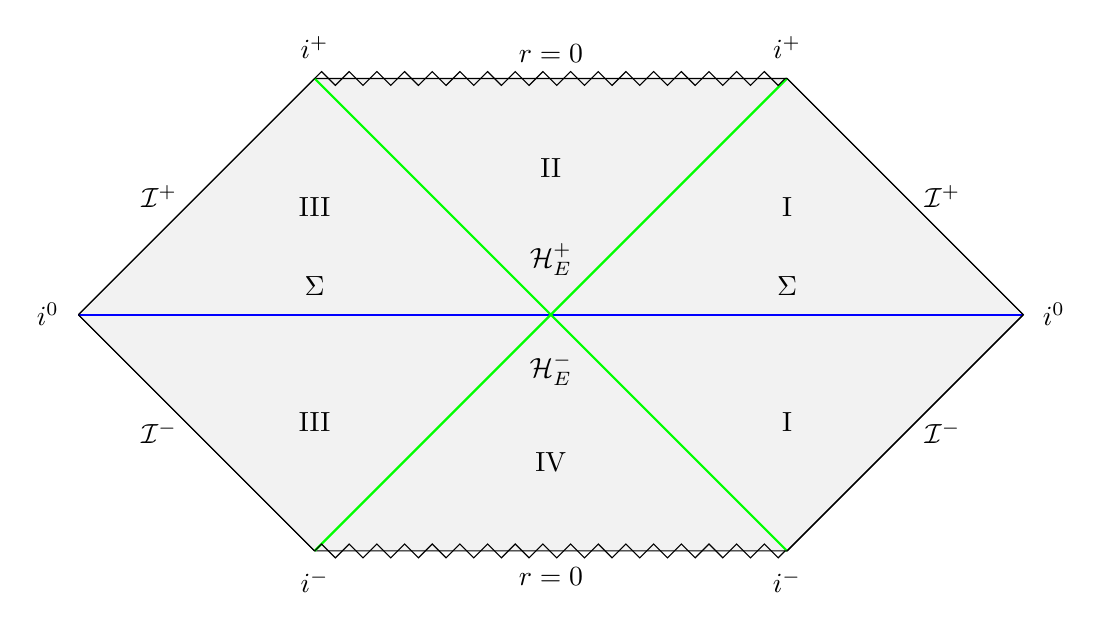
\begin{tikzpicture}
     \draw[fill=gray!10]    (-6,0) -- ++(3,3) -- ++(6,0) -- ++(3,-3)-- ++(-3,-3)-- ++(-6,0) -- ++(-3,3) ;   
         \draw[blue,thick] (-6,0) -- (6,0);
            \draw[green,thick] (-3,-3) -- (3,3);
                                                \draw[green,thick] (-3,3) -- (3,-3);
                                                \draw[decorate,decoration=zigzag]  (-3,3) -- (3,3)
    node[midway, above, inner sep=2mm] {$r=0$};
      \draw[decorate,decoration=zigzag]  (-3,-3) -- (3,-3)
    node[midway, below, inner sep=2mm] {$r=0$};
    \draw (3,3) -- (6,0);
\draw (3,-3) -- (6,0);
\draw (-3,-3) -- (-6,0);
\draw (-3,3) -- (-6,0);
          \node[label=above:$\mathcal{H}_E^+$]  at (0,0.25) {};
                                     \node[label=below:$\mathcal{H}_E^-$]  at (0,-0.25) {};
                                         \node[label=above:II]  at (0,1.5) {};
                                     \node[label=below:IV]  at (0,-1.5) {};
                                          \node[label=above:$\Sigma$]  at (-3,0) {};
                                                                  \node[label=above:$\Sigma$]  at (3,0) {};
                                                                    \node[label=below:III]  at (-3,-1) {};
                                                                      \node[label=above:III]  at (-3,1) {};
                                                                      \node[label=below:I]  at (3,-1) {};
                                                                       \node[label=above:I]  at (3,1) {};
                                     \node[label=right:$\mathcal{I}^+$]  at (4.5,1.5) {};
                                 \node[label=left:$\mathcal{I}^+$]  at (-4.5,1.5) {};    
                      \node[label=right:$\mathcal{I}^-$]  at (4.5,-1.5) {};
                                 \node[label=left:$\mathcal{I}^-$]  at (-4.5,-1.5) {};      
                                       \node[label=right:$i^0$]  at (6,0) {}; 
                                           \node[label=left:$i^0$]  at (-6,0) {}; 
                        \node[label=above:$i^+$]  at (3,3) {};
                          \node[label=above:$i^+$]  at (-3,3) {};
         \node[label=below:$i^-$]  at (3,-3) {};
                          \node[label=below:$i^-$]  at (-3,-3) {};                                               
    \end{tikzpicture}
\end{center}
\emph{Penrose diagram of the maximally extended Schwarzschild solution with $m>0$. This solution coincides with the maximal Cauchy development (marked in light grey) of a generic two-sided Cauchy surface $\Sg$ with suitable initial data, drawn as a horizontal blue line.  Thus the Cauchy horizon $\mathcal{H}^{\pm}_C$ is empty. The upper two green lines form the future event horizon $\mathcal{H}^+_E$ of the black hole area, which is the upside-down upper triangle (labeled region II), whereas the lower two green lines form the past event horizon $\mathcal{H}^-_E$ of the white hole area, i.e.\ the  lower triangle (region IV). The right-hand diamond is region I, the left-hand diamond is region III.
Fd causal curves cannot \emph{leave} region II and they cannot 
\emph{enter} region IV.
}\smallskip

 Both cosmic censorship conjectures hold in both versions (i.e.\ Penrose and \pde):
\begin{itemize}
\item  \emph{Weak  cosmic censorship.} Penrose:  $\Sg$ is a Cauchy surface for $J^-(\CI^+)$, making it globally hyperbolic.\footnote{Alternatively: any \emph{incomplete} future inextendible timelike curve $\gm$  must crash in the upper $r=0$ singularity. Hence $I^-(\gm)$ lies partly in region II, which is disjoint from $J^-(\CI^+)$, so that $I^-(\gm)\nsubseteq J^-(x)$  for all $x\in J^-(\CI^+)$.} \pde: each component of $\CI^+$ ends  at timelike infinity and hence all its null geodesics are future complete (as confirmed by explicit parametrization and computation). 
\item \emph{Strong  cosmic censorship.}   Penrose: Kruskal space-time is globally hyperbolic (since the causal structure
of the diagram  is such that the line $\Sg$ represents a Cauchy surface).
 \pde: For smooth extensions
 Remark 5.45 on page 155 of O'Neill (1983) or Proposition 4.4.3 in  Chru\'{s}ciel (2020) plus a detailed study of the geodesics shows that  Kruskal space-time is metrically
 inextendible.\footnote{ If for any maximally extended timelike geodesic $\gm:[0,b)\raw M$ in $M$ there is a curvature invariant (such as $R$ or $R^{\rh\sg\mu\nu}R_{\rh\sg\mu\nu}$, etc.)
  that blows up as $\gm(t)\raw b$, then $(M,g)$ is  inextendible. 
 See O'Neill (1983), Chapter 13, for a study of Kruskal geodesics,  proving the antecedent.
Sbierski (2018ab) proves that Kruskal space-time is inextendible even in $C^0$.}
\end{itemize}

 \noindent However, for $m<0$ Kruskal, Reissner--Nordstr\"{o}m, and Kerr, differences arise between the Penrosian and the \pde\ perspectives, since in these cases the  maximal (analytic) solutions, deemed unphysical by the \pde\ aficionados, differ from the \mghd\ of the pertinent initial data. In particular, although (curvature) singularities are not part of space-time in any case,
they can at least be drawn as boundaries in the maximal solutions, where they lie behind a Cauchy horizon. But precisely for that reason  singularities are outside any kind of scope of the corresponding \mghd.  Here are the Penrose diagrams:
 %\begin{small}
\begin{center}
\begin{minipage}{0.4\textwidth}
  \centering
   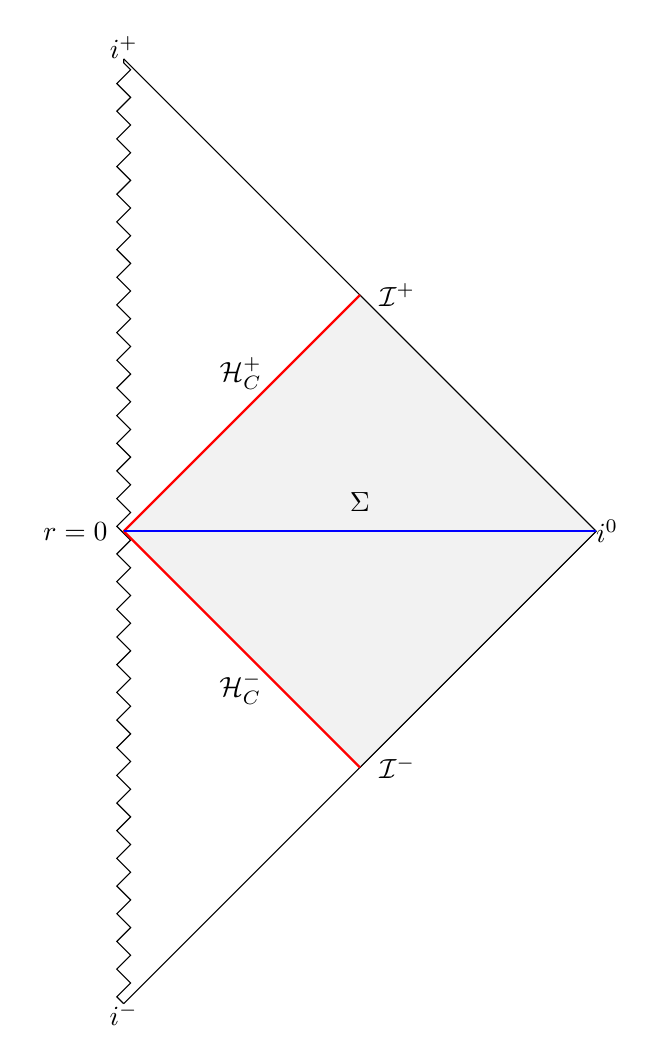
\begin{tikzpicture}
\draw (0,-6) -- (6,0);
\draw (6,0) -- (0,6);
\draw[decorate,decoration=zigzag]  (0,-6) -- (0,6)
    node[midway, left, inner sep=2mm] {$r=0$};
       \node[label=right:$\mathcal{I}^+$]  at (3,3) {};
            \node[label=right:$\mathcal{I}^-$]  at (3,-3) {};
               \node[label=left:$\mathcal{H}_C^+$]  at (2.0,2.0) {};
               \node[label=left:$\mathcal{H}_C^-$]  at (2.0,-2.0) {};
                     \node[label=right:$i^0$]  at (5.75,0) {}; 
                        \node[label=above:$i^+$]  at (0,5.75) {};
                         \node[label=below:$i^-$]  at (0,-5.75) {};  
                  \draw[fill=gray!10]    (0,0) -- ++(3,3) -- ++(3,-3) -- ++(-3,-3)-- ++(0,-0);                            
            \draw[red,thick] (0,0) -- (3,3);
             \draw[red,thick] (0,0) -- (3,-3);
               \draw[blue,thick] (0,0) -- (6,0);
                    \node[label=above:$\Sigma$]  at (3,0) {};
    \end{tikzpicture}
\end{minipage}%
\begin{minipage}{0.1\textwidth}
\mbox{} \end{minipage}%
\begin{minipage}{0.4\textwidth}
  \centering
   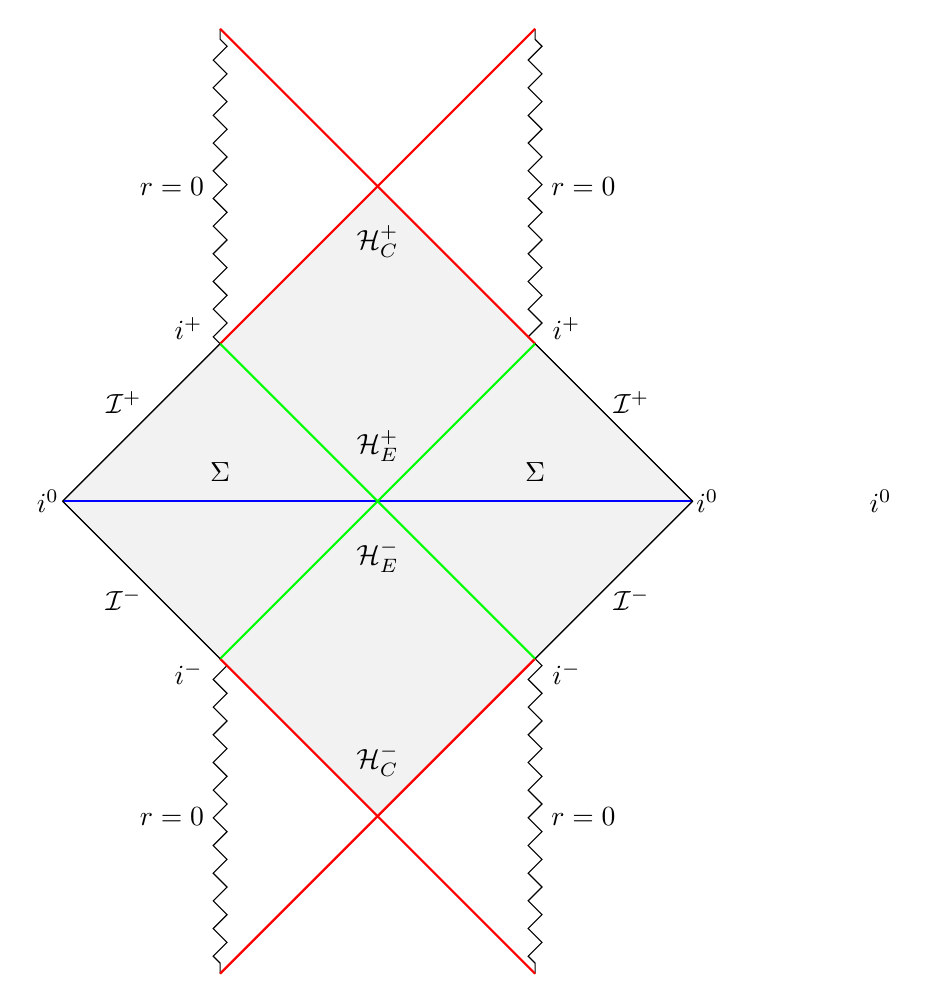
\begin{tikzpicture}
    \draw[fill=gray!10]    (-4,0) -- ++(4,4) -- ++(4,-4) -- ++(-4,-4)-- ++(-4,4);   
   \draw[decorate,decoration=zigzag]  (2,2) -- (2,6)
    node[midway, right, inner sep=2mm] {$r=0$};
    \draw[decorate,decoration=zigzag]  (-2,2) -- (-2,6)
    node[midway, left, inner sep=2mm] {$r=0$};
       \draw[decorate,decoration=zigzag]  (2,-2) -- (2,-6)
    node[midway, right, inner sep=2mm] {$r=0$};
    \draw[decorate,decoration=zigzag]  (-2,-2) -- (-2,-6)
    node[midway, left, inner sep=2mm] {$r=0$};
               \draw[red,thick] (2,2) -- (-2,6);
                    \draw[red,thick] (-2,2) -- (2,6);
                               \node[label=above:$\mathcal{H}_E^+$]  at (0,0.25) {};
                                     \node[label=below:$\mathcal{H}_E^-$]  at (0,-0.25) {};
                                    \draw[blue,thick] (-4,0) -- (4,0);
                                          \draw[green,thick] (-2,2) -- (0,0);
                                                \draw[green,thick] (2,2) -- (0,0);
                                                         \node[label=above:$\Sigma$]  at (-2,0) {};
                                                                  \node[label=above:$\Sigma$]  at (2,0) {};
                                    \draw (-2,2) -- (-4,0);{};  
                                       \draw (2,2) -- (4,0);{};    
            \node[label=below:$\mathcal{H}_C^+$]  at (0,3.75) {};
                      \node[label=right:$\mathcal{I}^+$]  at (2.75,1.25) {};
                                 \node[label=left:$\mathcal{I}^+$]  at (-2.75,1.25) {};    
               \node[label=above:$\mathcal{H}_C^-$] at (0,-3.75) {};
                      \node[label=right:$\mathcal{I}^-$]  at (2.75,-1.25) {};
                                 \node[label=left:$\mathcal{I}^-$]  at (-2.75,-1.25) {};    
                \draw[red,thick] (-2,-2) -- (2,-6);
                    \draw[red,thick] (2,-2) -- (-2,-6);
                     \draw[green,thick] (-2,-2) -- (0,0);
 \draw[green,thick] (2,-2) -- (0,0);         
            \draw (-2,-2) -- (-4,0);{};  
                                       \draw (2,-2) -- (4,0);{};   
                     \node[label=right:$i^0$]  at (6,0) {}; 
                        \node[label=above:$i^+$]  at (2.4,1.8) {};
                          \node[label=above:$i^+$]  at (-2.4,1.8) {};
         \node[label=below:$i^-$]  at (2.4,-1.8) {};
                          \node[label=below:$i^-$]  at (-2.4,-1.8) {};   
                                     \node[label=right:$i^0$]  at (3.8,0) {};
 \node[label=left:$i^0$]  at (-3.8,0) {};                                                   
    \end{tikzpicture}
\end{minipage}
\end{center}
%\end{small}
\smallskip


\emph{\hi{Left picture:} Penrose diagram of $m<0$ Schwarzschild, or supercharged Reissner--Nordstr\"{o}m  ($e^2>m^2>0$), or fast  Kerr ($a^2>m^2>0$). These solutions have a singularity at $r=0$, but unlike the $m>0$ Kruskal case it is not shielded by an event horizon. Instead, the red lines labeled $\mathcal{H}_C^-$ and $\mathcal{H}_C^+$ are past and future Cauchy horizons with respect to the blue line, indicating a maximal spacelike surface whose initial data give rise to the metrics in question and whose maximal Cauchy development is the grey area. }
\smallskip

\emph{\hi{Right picture:}  Penrose diagram of subcritical Reissner--Nordstr\"{o}m  ($0<e^2<m^2$), whose event and Cauchy horizons (despite the different structure of the singularity) also resemble those of slowly rotating Kerr ($0<a^2<m^2$). The  maximal Cauchy development of the pertinent initial data given on the maximal spacelike hypersurface represented by the blue line labeled $\Sg$ is again colored in grey. It contains past and future event horizons labeled  $\mathcal{H}_E^-$ and $\mathcal{H}_E^+$, drawn in green, but unlike  the $m>0$ Schwarzschild case  the singularity they are supposed to shield cannot be reached directly from the  maximal Cauchy development, which is bounded by the various fictitious boundaries $\CJ^{\pm}$, $i^{\pm}$, and $i^0$, which lie at infinity, as well as by the Cauchy horizons  $\mathcal{H}_C^{\pm}$, drawn in red, which can be reached in finite proper time.\footnote{ 
This diagram can be infinitely extended  in both directions (Hawking \& Ellis, 1973, pp.\ 158, 165): to the north, another grey area folds inside the upper two red line segments, and similarly to the south, \emph{et cetera}, but we do \emph{not} do so here.}}

\noindent  Despite the different space-times they apply to, the outcomes of the Penrosian version and the \pde\ version of both weak and strong cosmic censorship are once again the same, \emph{mutatis mutandis}:\footnote{For $m<0$ Kruskal the initial data are not complete in this case, so strictly speaking the cosmic censorship conjectures do not apply here and their falsity is unimportant. Nonetheless, they can be stated and the comparison is instructive.} 
\begin{itemize}
\item  $m<0$ Kruskal (etc.): For the Penrosian total space-time the difference between weak and strong  cosmic censorship  fades since
 $J\inv(\CI^+)=M\cup\CI^+$, which, like $M$ itself is not globally hyperbolic: wherever one tries to place a partial Cauchy surface $\Sg$ (such as the blue line), above the surface  inextendible causal curves can be drawn that enter $i^+$ or $\CI^+$ in the future and enter the singularity at $r=0$ in the past, without  crossing $\Sg$. Similarly, below $\Sg$ one may draw  inextendible causal curves converging to the
 singularity in the future, and to  $i^-$ or $\CI^-$ in the past, which once again do not cross $\Sg$. Thus neither weak nor strong cosmic censorship  holds for this space-time.
 
The \pde\ picture applies to the grey area, which is the \mghd\ of the initial data given on the blue line marked $\Sg$  in the left-hand Penrose diagram. Then
 weak cosmic censorship fails because future null infinity $\CI^+$ is clearly incomplete: null geodesics terminate at the Cauchy horizon (where they ``fall off' space-time) and hence are incomplete. On the other hand, strong cosmic censorship fails because the grey space-time, though globally hyperbolic (in contrast with the entire space as we have just seen), is evidently (smoothly--even analytically) extendible, namely by the total space.  Though they do not coincide, we see  that strong and weak cosmic censorship are closely related: future incompleteness of null geodesics at null infinity 
happens because the \mghd\ is extendible.
 
 \item  Subcritical Reissner--Nordstr\"{o}m  ($0<e^2<m^2$):  for both Penrose and the \pde\ people strong cosmic censorship fails whereas the weak version holds.
  In the Penrosian version the total space  fails to be globally hyperbolic because of the part above the grey area (i.e.\ beyond the future Cauchy horizon $\mathcal{H}_C^+$): one has past-directed inextendible causal curves that (backwards in time) end up in the singularity and hence never cross $\Sg$ (e.g.\ those crossing the upper left, NW-pointing red line from N to SW). 
  Morally, weak  cosmic censorship  holds because of the future event horizon $\mathcal{H}_E^+$, which shields the upper $r=0$ singularity above it, 
  but legally this is only the case if we stop the Penrose diagram at the past Cauchy horizon $\mathcal{H}_C^-$, as we have  done in drawing the picture (for otherwise causal curves below it may crash at the  lower $r=0$ singularity and hence never reach $\Sg$). 
  
  The \pde\ view is cleaner here: roughly speaking, as in the $m>0$ Kruskal or Schwarzschild case (but unlike the $m<0$ case) future null infinity $\CI^+$ ends at future timelike infinity $i^+$ and hence is complete, so that weak  cosmic censorship holds. Strong  cosmic censorship, on the other hand, fails because the \mghd\ (marked in grey) is clearly extendible (namely into the Penrosian space-time!). 
\end{itemize}
More generally, if the strong Penrosian conjecture fails for some space-time $(M_P,g_P)$, then its lack of global hyperbolicity  typically occurs because $(M_P,g_P)$ is an extension of the \mghd\ $(M,g)$ of some given initial data, whose Cauchy surface $\Sg$ fails to be one for  $(M_P,g_P)$.
Similarly, if $J\inv(\CI^+)$ is not globally hyperbolic (so that there is a naked singularity), $M_P$ usually comes from extending some $(M,g)$, as above, whose Cauchy surface becomes a partial  Cauchy surface in $M_P$, with an associated future Cauchy horizon that cuts off $\CI^+\cap\til{M}$, causing its incompleteness.\footnote{However, these aren't rigorous deductions: there are pathological cases where strong cosmic censorship holds whilst the weak version fails. See the Penrose diagram at the end of \S 2.6.2 of Dafermos \& Rodnianski (2008) for an example.} 
As already mentioned, any counterexamples are believed to be ``non-generic'', assuming of course that the conjectures hold! 

Such reasoning, which applies to many case studies,  also suggests a compromise between the Penrosian and \pde\ versions of cosmic censorhsip: informally  one might say that, in physically reasonable space-times, weak cosmic censorship postulates the \emph{appearance and stability of event horizons}, whereas  strong cosmic censorship requires the \emph{instability and ensuing disappearance of Cauchy horizons}.
\section{Epilogue: Penrose's final state conjecture}\label{FSC}
In practice, the cosmic censorship conjectures are not put in the full  generality of either Penrose's own version as expressed by Theorem \ref{P79theorem} or of the \pde\ version as Definition \ref{CSfed1}, 
but are posed in the context of black holes as they are expected to occur in the universe, i.e.\ as described by something like the Kerr metric (at least outside its Cauchy horizon and more safely even outside its event horizon). As such, on the one hand
 they gain focus, but on the other hand they can be thought of as
 forming part of a broader  conjecture that also originated with Penrose himself and is often called the \emph{final state conjecture}:\footnote{This is sometimes stated somewhat differently, in that `generic asymptotically  flat vacuum initial data (\ldots) evolve to a solution which either disperses (in which case there are no black holes) or else eventually asymptotes to
  finitely many Kerr solutions (...) moving away from each other' (Coley, 2019, p.\ 78). See also the fascinating lecture by Klainerman (2014).
  }
 \begin{quote}
\begin{small}A body, or collection of bodies, collapses down to a size comparable to its Schwarzschild radius, after which a trapped surface can be found in the region surrounding the matter. Some way outside the trapped surface region is a surface which will ultimately be the absolute event horizon. But at present, this surface is still expanding somewhat. Its exact location is a complicated affair and it depends on how much more matter (or radiation) ultimately falls in. We assume only a finite amount falls in and that {\sc gic} is true. Then the expansion of the absolute event horizon gradually slows down to stationarity. Ultimately the field settles down to becoming a Kerr solution (in
the vacuum case) or a Kerr-Newman solution (if a nonzero net charge is trapped in the ``black hole''). (Penrose, 1969, pp.\ 1157--1158)
\end{small}
\end{quote}
Here {\sc gic} refers to what Penrose (1969) called the \emph{Generalized Israel Conjecture},\footnote{The reference is to Israel (1967, 1968). See Israel (1987), \S 7.9 and Thorne (1994), Chapter 7, for interesting history.}
which states that:
 \begin{quote}
\begin{small}
 if an absolute event horizon develops in an asymptotically flat space-time, then the solution exterior to this horizon approaches a Kerr-Newman solution asymptotically with time. (Penrose, 1969, pp.\ 1156)
\end{small}
\end{quote}
 In the stationary case, which is what Israel himself conjectured and proved under fairly restrictive assumptions, this would simply say that the solution exterior to this horizon \emph{equals} a Kerr-Newman solution. As such, the conjecture  is an outgrowth of what (following Wheeler) used to be called the ``no hair'' property of black holes, to the effect that stationary black holes (and eventually all black holes)
  are characterized by by just three parameters, viz.\ mass, angular momentum, and electric charge. As such, the final state conjecture incorporates not only weak cosmic censorship (notably in the compromise version suggested at the end of the previous section) but also what in the \pde\ literature is called \emph{Kerr stability},  as well as \emph{Kerr rigidity}. The former is
   the conjecture that generic  perturbations of the  initial data
 for the  Kerr metric lead to a \mghd\ that is close to the original one (at least outside the event horizon).\footnote{There is certain  numerical evidence for this (Zilh\~{a}o et al., 2014), but mathematical results so far are  preliminary (Dafermos,  Holzegel, \&  Rodnianski, 2019b; 
Giorgi, Klainerman, \& Szeftel, 2020), except for positive cosmological constant and small $a$  (Hintz \& Vasy, 2018), where the problem is solved. 
Even the Schwarzschild case is still open, despite impressive progress (Klainerman \& Szeftel, 2017; Dafermos,  Holzegel, \&  Rodnianski, 2019a).
} This would generalize the remarkable theorem on the stability of Minkowski space-time (Christodoulou \& Klainerman, 1993), which launched the modern era in \pde-oriented mathematical relativity. 
The latter  is a more modest version of the no-hair or black hole uniqueness theorems of Israel, Carter, Hawking, Robinson, and others,\footnote{These theorems are reviewed in Hawking \& Ellis (1973), \S 9.3, Carter (1979, 1986), Heusler (1996), Robinson (2009), Chru\'{s}ciel,  Lopes Costa, \& Heusler (2012), and Cederbaum (2019).  See also Cardoso \&  Gualtieri (2016) for possible  tests.
} where short of proving the stationary case of the above {\sc gic}, which requires unphysical analyticity assumptions, one tries to show that at least stationary solutions to Einstein's vacuum (electrovac) equations that are close to Kerr (--Newman) actually coincide with the latter.\footnote{See e.g.\
Alexakis,  Ionescu, \& Klainerman (2014) as well as the review by Ionescu \&  Klainerman (2015).}
\smallskip

In conclusion, ``the discovery that black hole formation is a robust prediction of the general theory of relativity'' still lies in the future as far as mathematical proof is concerned. Penrose's Nobel Prize was effectively awarded for a theorem and a conjecture, but it was fully deserved in every conceivable way!
\appendix
\section{A potted early history of ``black hole'' (by Erik Curiel)} 
In reply to a query in the penultimate draft of this paper concerning  the origin of the definitions $\mathcal{B}:= M\backslash J^-(\CI^+)$ of a black hole (region) and of the event horizon as its boundary $\mathcal{H}_E^+:=\p \mathcal{B}$, see 
\er{BHRWHR} and \er{defEHplus}, phrased as: `Such definitions are routinely used in e.g.\ Carter (1971a) and Hawking \& Ellis (1973), \S 9.2, but who stated them first?',  Erik Curiel very kindly supplied the following information.\footnote{As in the rest of the paper, single quotation marks below denote literal quotation whereas double ones are scare quotes.}  As we see, the question still remains somewhat open. A puzzling point is that
although Penrose himself would have been the obvious person to state these definitions mathematically, apparently he did not do so!
\begin{quote}
\begin{small}
Penrose (1968) defines (p.\ 188), an event horizon as the boundary of the chronological past of
a timelike curve (essentially the same definition, including the name, as given by Rindler 1956),
and notes (p.\ 206) that $r = 2M$ in Schwarzschild is one. The term ``black hole'' does not appear
in that essay, nor any definition remotely like `the complement of the causal past of future null
infinity'. Given the magisterial depth and encyclopedic scope of that essay, I must conclude that
the definition was not then yet extant. Penrose (1969) does use the term ``black hole'' (the first use
of it I know in the general relativity literature, though it reportedly was used in the early 1960s by
Dicke in discussion with a popular science writer), but he always encloses it in scare quotes, leading
me to believe that the name and the general concept both were still inchoate. This is buttressed
by the fact that he does give here (p.\ 1146, footnote 3) the classic definition of an `absolute event
horizon' (the boundary of the chronological past of future null infinity), but he does not explicitly
link it to the term ``black hole''. That is the first appearance of the classic definition I know of in
the literature.

Ruffini and Wheeler gave a series of lectures in September 1969 at the \emph{Interlaken Colloquium on
the Significance of Space Research for Fundamental Physics} (Interlaken, Switzerland), one of which
was entitled `Black Holes', at least according to the expanded version of the lectures published as
Ruffini and Wheeler (1971a), from which Ruffini and Wheeler (1971b) was adapted. This is the first
use of the term I have been able to find recorded in a public forum in the relativity community.
They explain the idea in informal, intuitive terms. Bardeen (1970), received 23 January 1970,
has ``black hole'' in the title, the first publication I know of to do so. He introduces ``black hole''
using scare quotes and equates it with a `collapsed object'. Israel (1971), originally read at 
 the \emph{Gwatt Seminar on the Bearings of
Topology upon General Relativity} on 19 May 1970, uses ``black hole'' without defining it, but it is clear from context that he
means something like `system that quickly settles down so that its exterior is modeled by the Kerr
solution'.  Christodoulou (1970), received 17 September 1970, uses the term without blushing,
not even an informal gloss given for its meaning. He simply begins by talking of a `black hole
[with] angular momentum' without even citing Kerr (1963). Three papers then appear in 1971
with ``black hole'' in the title, Penrose and Floyd (1971), received 16 December 1970, Carter (1971),
received 18 December 1970, and Hawking (1971), received 11 March 1971. They are the only other
papers from 1971 I can find related to the topic whose authors plausibly could have proposed
the classic definition. Penrose and Floyd (1971) uses scare-quotes around the first use of ``black
hole''; their discussion relies only on the event horizon and ergosphere (which they refer to as the
`stationary limit') defined by the Kerr metric, with no attempt at (or mention of the possibility
of) generalization. Carter (1971) does not give a formal definition of ``black hole'', but he does give
an informal definition of `domain of outer communication', and says (p.\ 331) that `\! ``black holes''
[are] regions of space-time beyond the domain of outer communication.' Note the scare-quotes.
Hawking (1971) uses scare-quotes as well, going out of his way to assimilate the idea of a black
hole to one more widely known (`there are initially two collapsed objects or ``black holes''', p.\ 1345).
He also comes achingly close to defining a black hole as a connected component of the complement
of the causal past of future null infinity, but never quite does it. He rather says things like, 
`On $\Sg_i$ [a spacelike hypersurface], there will be two separate regions, $B_1$ and $B_2$ which contain closed,
trapped surfaces (\ldots)  Just outside $B_1$ and $B_2$ will be two two-spheres which are the intersection
of $\dot{J}^-(\CI^+)$ with $\Sg_i$.' The first explicit definition I know of ``black hole'' as `connected component of the complement of the causal past of future null infinity' is in Hawking (1972). But I am not
confident that I have found all relevant sources in the literature; even if I have, one cannot be
confident based only on this that Hawking was the one who finally put all the pieces together.
 
(Erik Curiel, private communication, January 6, 2021, reprinted with permission)
\end{small}
\end{quote}
\newpage

\noindent \textbf{Acknowledgement.} This paper grew out of a seminar in honour of Roger Penrose and his Nobel Prize at Nijmegen on October 28th, 2020, at the kind invitation of Timothy Budd. The author is grateful to Carlo Rovelli for encouragement to publish it, as well as to B\'{e}atrice Bonga, Jeremy Butterfield, Erik Curiel, John Earman,  Dejan Gajic, and Dennis Lemkuhl for helpful feedback on this talk and/or earlier drafts.
\smallskip

\addcontentsline{toc}{section}{References}
\begin{small}
\begin{thebibliography}{99}
\item[]  Adamo, T.M.,  Newman, E.T.,  Kozameh C. (2012). Null geodesic congruences, asymptotically-flat spacetimes and their physical interpretation.  \emph{Living Reviews in Relativity} 15 (1).
\item[]  Alaee, A.,  Lesourd, M., Yau, S.-T. (2019). A localized spacetime Penrose inequality and horizon detection with quasi-local mass. \texttt{arXiv:1912.01581}. 
\item[]  Alexakis, S.,  Ionescu, A.D.,  Klainerman, S. (2014). Rigidity of stationary black holes with small angular momentum on the horizon. \emph{Duke Mathematical Journal}  14, 2603--2615.
\item[] Ashtekar, A. (1980). Asymptotic structure of the gravitational field at spatial infinity.
 \emph{General Relativity and Gravitation: One Hundred Years After the Birth of Albert Einstein}, Vol.\ 2.
 Held, A., ed., pp.\ 37--70 (Plenum). 
\item[] Ashtekar, A. (2015). Geometry and physics at null infinity. \texttt{arXiv:1409.1800}.
 \item[]  Ashtekar, A.,  Bonga, B., Kesavan, A.  (2015) . Asymptotics with a positive cosmological constant: I. Basic framework. \emph{Classical and Quantum Gravity} 32, 025004. 
  \item[]  Ashtekar, A.,   Magnon, A. (1984). 
  Asymptotically anti-de Sitter space-times.  \emph{Classical and Quantum Gravity} 1, L39--L44. 
\item[]   Athanasiou, N.,  Lesourd, M. (2020).  Construction of Cauchy data for the dynamical formation of apparent horizons and the Penrose Inequality. \texttt{arXiv:2009.03704}.
\item[]  B\"{a}r, C., Ginoux, N., and Pf\"{a}ffle, F. (2007). \emph{Wave Equations on Lorentzian Manifolds and Quantization}
(European Mathematical Society). 
\item[]  Bardeen, J. (1970). Kerr metric black holes. \emph{Nature} 226, 64--65.
\item[] Bieri, L. (2018). Black hole formation and stability: a mathematical investigation. \emph{Bulletin of the American Mathematical Society (N.S.)} 55, 1--30.
\item[] Burtscher, A.Y. (2020). Initial data and black holes for matter models. \emph{
Hyperbolic Problems: Theory, Numerics, Applications. AIMS Series in  Applied Mathematics}  10, 336--345.
\item[] Burtscher, A.Y.,  LeFloch, P.G. (2014). The formation of trapped surfaces in spherically-symmetric Einstein--Euler
spacetimes with bounded variation. \emph{Journal de Math\'{e}matiques Pures et Appliqu\'{e}es} 102 1164--1217.
\item[] Butterfied, J. (2011). Less is different: Emergence and reduction reconciled.
\emph{Foundations of Physics}  41, 1065--1135
\item[]  Candela, A.M.,  Flores, J.L., S\'{a}nchez, M.  (2010).
Global hyperbolicity and Palais--Smale condition for action functionals in stationary spacetimes.
\emph{Advances in Mathematics} 218, 515--536.
\item[]  Cardoso, V.,  Gualtieri, L. (2016). Testing the black hole `no-hair' hypothesis. \emph{Classical and Quantum Gravity}
33, 174001.
\item[] Carter, B. (1971a). Causal structure in space-time. \emph{General Relativity and Gravitation} 1, 349--391.
\item[] Carter, B. (1971b). Axisymmetric black hole has only two degrees of freedom. \emph{Physical Review
Letters} 26, 331--333.
\item[] Carter, B. (1973). Black hole equilibrium states. Part I: Analytic and geometric properties of the Kerr solution.
\emph{Black Holes--Les astres occlus}, eds.\  De Witt, B., DeWitt-Morette, C., pp.\ 61--124 (Gordon and Breach).
Reprinted in \emph{General Relativity and Gravitation} 41, 2873--2938 (2009).
\item[] Carter, B. (1979). The general theory of the mechanical, electromagnetic and thermodynamic properties of black holes.  \emph{General Relativity: An Einstein Centenary Survey}, eds.\ 
S.W. Hawking \& W. Israel, pp.\ 294--369 (Cambridge University Press). 
\item[] Carter, B. (1986). Mathematical foundations of the theory of relativistic stellar and black hole configurations.
\emph{Gravitation in Astrophysics (Carg\`{e}se 1986)}, eds.\ Carter, B., Hartle, J.B., 
pp.\ 63--122 (Plenum Press). 
\item[]  Cederbaum, C. (2019). \emph{Static black hole uniqueness theorems. Lectures 1--4. ICTP School of Geometry and Gravity}. 
\verb#https://www.youtube.com/watch?v=hf4qIiGVwLk# etc.
\item[]  Chesler, P.M.,  Narayan, R.,  Curiel, E. (2020). Singularities in Reissner--Nordstr\"{o}m black holes.
 \emph{Classical and Quantum Gravity} 37, 025009.  
\item[] Choquet-Bruhat, Y. (1967).  Hyperbolic partial differential equations on a manifold.
\emph{Batelle Rencontres: 1967 Lectures in Mathematics and Physics}, eds. 
 C. DeWitt and J.A. Wheeler, pp.\ 84--106 (W.A. Benjamin). 
 \item[]  Choquet-Bruhat, Y. (2009). \emph{General Relativity and the Einstein Equations} (Oxford University Press). 
\item[]  Choquet-Bruhat, Y. (2014). Beginnings of the Cauchy problem, \texttt{arXiv:1410.3490}.
\item[] Choquet-Bruhat, Y. (2018). \emph{A Lady Mathematician in this Strange Universe: Memoirs} (World Scientific).
\item[] Choquet-Bruhat, Y.,  Geroch, R. (1969). Global aspects of the Cauchy problem in general relativity.
 \emph{Communications in Mathematical Physics} 14, 329--335.
 \item[]
 Christodoulou, D. (1970). Reversible and irreversible transformations in black-hole physics. \emph{Physical
Review Letters} 25, 1596--1597.
  \item[] Christodoulou, D.  (1991). The formation of black holes and singularities in spherically symmetric gravitational collapse. 
  \emph{Communications in Pure and Applied Mathematics} 44, 339--373.
 \item[] Christodoulou, D. (1999a). On the global initial value problem and the issue of singularities.
\emph{Classical and Quantum Gravity} 16, A23--A35. 
 \item[] Christodoulou, D. (1999b). The instability of naked singularities in the gravitational collapse of a scalar field.
 \emph{ Annals of Mathematics} 149, 183--217. 
 \item[]  Christodoulou, D. (2009). \emph{The Formation of Black Holes in General Relativity} (European Mathematical Society). 
 \item[] Christodoulou, D., Klainerman, S. (1993). \emph{The Global Nonlinear Stability of the Minkowski Space}
(Princeton University Press). 
 \item[] Chru\'{s}ciel, P.T.  (1992). On uniqueness in the large of solutions of Einstein's equations (``Strong Cosmic Censorship''). \emph{Mathematical Aspects of Classical Field Theory. Contemporary Mathematics} 132, 235--274.
 \item[]  Chru\'{s}ciel, P.T. (2011), Elements of causality theory. \texttt{arXiv:1110.6706}.
\item[]  Chru\'{s}ciel, P.T. (2019). \emph{Elements of General Relativity} (Springer). 
\item[]  Chru\'{s}ciel, P.T. (2020). \emph{Geometry of Black Holes} (Oxford University Press). 
\item[]   Chru\'{s}ciel, P.T., Delay, E., Galloway,  G.J., Howard, R. (2001). 
Regularity of horizons and the area theorem.
\emph{Annales Henri Poincar\'{e}} 2, 109--178. 
\item[]   Chru\'{s}ciel, P.T., Galloway, G.J.,  Pollack, D. (2010).
Mathematical general relativity: A sampler. \emph{Bulletin of the American Mathematical Society} 47, 567--638.
\item[] Chru\'{s}ciel, P.T.,  Lopes Costa, J.,  Heusler, M. (2012).
Stationary black holes: uniqueness and beyond. \emph{Living Reviews in Relativity} 15 (7).
\item[]  Chru\'{s}ciel, P.T., Paetz, T.T. (2015). Characteristic initial data and smoothness of Scri. I. Framework and results.
\emph{ Annales Henri Poincar\'{e}} 16, 2131--2162.
\item[]   Clarke,  C.J.S. (1993). \emph{The Analysis of Space-Time Singularities} (Cambridge University Press).
\item[] Coley, A.A. (2019). Mathematical general relativity. \emph{General Relativity and Gravitation} 51, 78--112.
\item[] Curiel, E. (1999).  The analysis of singular spacetimes. \emph{Philosophy of Science} 66, S119--S145. 
Revised and extended version at \verb#http://strangebeautiful.com/phil-phys.html#.
\item[] Curiel, E. (2019a). Singularities and Black Holes. \emph{The Stanford Encyclopedia of Philosophy (Spring 2019).}\\ \verb#https://plato.stanford.edu/archives/spr2019/entries/spacetime-singularities/#.
\item[] Curiel, E. (2019b). The many definitions of a black hole. \emph{Nature Astronomy} 3, 27--34.
 \item[] Dafermos, M. (2003). Stability and instability of the Cauchy horizon for the spherically symmetric Einstein--Maxwell-scalar field equations. \emph{Annals of Mathematics} 158, 875--928. 
 \item[] Dafermos, M. (2012). The formation of black holes in General Relativity [after D. Christodoulou]
\emph{S\'{e}minaire Bourbaki} 64, no.\ 1051. \verb#https://www.dpmms.cam.ac.uk/~md384/expose-chr.pdf#.
 \item[] Dafermos, M. (2013). The geometry and analysis of black hole spacetimes in general relativity ({\sc eth} \emph{Nachdiplom} lectures). \verb#https://www.dpmms.cam.ac.uk/~md384/Ravello_Lectures_1.pdf#.
  \item[] Dafermos, M. (2014a). Black holes without spacelike singularities. 
   \emph{Communications in Mathematical Physics} 332, 729--
 \item[] Dafermos, M. (2014b). The mathematical analysis of black holes in general relativity. 
\emph{Proceedings of the ICM, 2014}, \verb#https://www.dpmms.cam.ac.uk/~md384/ICMarticleMihalis.pdf#.
 \item[] Dafermos, M. (2017). The cosmic censorship conjectures in classical general relativity. \verb#https://www.youtube.com/watch?v=ZBYAbejIvB4#.
  \item[] Dafermos, M. (2019).
 The cosmic censorship conjectures in general relativity  (ICTP School on Geometry and Gravity). 
  Lecture 1:  \verb#https://www.youtube.com/watch?v=Lg1Cetf7V9I#. 
Lecture 2:  \verb#https://www.youtube.com/watch?v=SoRhBSt_mN0#.
  \item[] Dafermos, M., Holzegel, G., Rodnianski, I. (2019a).
  The linear stability of the Schwarzschild solution to gravitational perturbations. \emph{Acta Mathematica} 222, 1--214. 
    \item[] Dafermos, M., Holzegel, G., Rodnianski, I. (2019b).
Boundedness and decay for the Teukolsky equation on Kerr spacetimes I: The Case $|a|\ll M$. 
\emph{Annals of PDE} 5:2. 
  \item[] Dafermos, M., Luk, J. (2017). The interior of dynamical vacuum black holes I: The $C^0$-stability of the Kerr Cauchy horizon. \texttt{arXiv:1710.01722}.
  \item[] Dafermos, M., Rodnianski, I. (2008). Lectures on black holes and linear waves. \texttt{arXiv:0811.0354}.
  \item[] 
Dias, O.J.C.,  Reall, H.S., Santos, J.E. (2018).
 Strong cosmic censorship: taking the rough with the smooth. \emph{Journal of High Energy Physics} 1. \verb#https://doi.org/10.1007/JHEP10(2018)001#.
\item[]  Earman, J. (1995).  \emph{Bangs, Crunches, Whimpers, and Shrieks: Singularities and Acausalities in Relativistic Spacetimes} (Oxford University Press).
\item[]  Earman, J. (1996). Tolerance for spacetime singularities. \emph{Foundations of Physics} 26, 623--640.
\item[] Earman, J. (1999). The Penrose--Hawking singularity theorems: History and implications. \emph{The Expanding Worlds of General Relativity (Einstein Studies Vol.\ 7)}, eds.\ Goenner, H., Renn, J., Ritter, T., Sauer, T., pp.\ 236--267
(Birkh\"{a}user). 
\item[]  Earman, J. (2004). Curie's Principle and spontaneous symmetry breaking, \emph{International Studies in  Philosophy of Science} 18, 173--198. 
\item[]  Earman, J. (2007). Aspects of determinism in modern physics.  \emph{Handbook of
the Philosophy of Science. Vol. 2: Philosophy of Physics, Part B}, eds.\   Butterfield, J., Earman, J.,
 pp.\ 1369--1434 (North-Holland/Elsevier).
\item[] Earman, J.,  Eisenstaedt, J. (1999). Einstein and Singularities. \emph{Studies in History and Philosophy of Modern Physics} 30, 185--235.
\item[] Einstein, A. (1915), Die Feldgleichungen der Gravitation,
\emph{Sitzungsberichte der K\"{o}niglich Preu\ss ischen Akademie der Wissenschaften (Berlin)} 844--847.
\item[] Einstein, A. (1918). \"{U}ber Gravitationswellen. \emph{Sitzungsberichte der K\"{o}niglich Preu\ss ischen Akademie der Wissenschaften (Berlin)} 154--167.
\item[] Einstein, A. (2002),   \emph{The Collected Papers of Albert Einstein, Vol.\ 7: The Berlin Years: Writings, 1918--1921},
eds.\ M. Janssen \emph{et al} (Princeton University Press). 
\\  \verb#https://einsteinpapers.press.princeton.edu/vol7-doc/#. 
\item[]  Eisenstaedt, J. (1993).  Lema\^{i}tre and the Schwarzschild solution.
\emph{The Attraction of Gravitation: New Studies in the History of General Relativity}, eds.\
Earman, J.,  Janssen, M.,  Norton, J.D., pp.\ 353--389  (Birkh\"{a}user). 
\item[]  Ellis, G.F.R. (2014). Stephen Hawking's 1966 Adams Prize Essay.  \emph{European Journal of Physics H} 
39, 403--411. 
        \item[] Event Horizon Telescope Collaboration (2019). First M87 event horizon telescope results. V. Physical origin of the asymmetric ring. \emph{The Astrophysical Journal Letters} 875:L5, 1--31.
\item[] Falcke, H. (2020). \emph{Licht im Dunkeln} (Klett--Cotta). 
\item[]  Finkelstein, D. (1958). Past-future asymmetry of the gravitational field of a point particle.
 \emph{Physical Review} 110, 956--967. 
 \item[] Franklin, A.D. (2017). Is seeing believing? Observation in physics. \emph{Physics in Perspective} 19, 321--423. 
\item[] Frauendiener, J. (2000). Conformal infinity.  \emph{Living Reviews in Relativity} 3 (4). 
\item[]  Friedrich, H. (2004). Smoothness at null infinity and the structure of initial data.
\emph{The Einstein Equations and the Large Scale Behavior of Gravitational Fields}, eds.\ 
Friedrich, H., Chru\'{s}ciel, P.T., pp.\ 121--203 (Springer).
\item[]  Friedrich, H. (2011). Editorial note to: Roger Penrose, Conformal treatment of infinity.  \emph{General Relativity and Gravitation} 43, 897--900.
\item[]  Friedrich, H. (2018). Peeling or not peeling--Is that the question?
\emph{Classical and Quantum Gravity} 35, 083001. 
  \item[]  Gajic, D., Luk, J. (2019). 
The interior of dynamical extremal black holes in spherical symmetry. \emph{Pure and Applied Analysis} 1, 263--326. 
  \item[]  Geroch, R.   (1968). What is a singularity in General Relativity? \emph{Annals of Physics (N.Y.)} 48, 526--540.
  \item[]  Geroch, R.   (1970). Domain of dependence, \emph{ Journal of Mathematical Physics} 11, 437--449.
    \item[]  Geroch, R.   (1977). Asymptotic structure of space-time. \emph{Asymptotic Structure of Space-Time}, eds.\ Esposito, F.P., Witten, L., pp.\ 1--105  (Plenum). 
      \item []  Geroch, R., Horowitz, G. (1978).
Asymptotically simple does not imply asymptotically Minkowskian. \emph{Physical Review Letters} 40, 203--206. 
    \item []  Geroch, R., Kronheimer, E.H.,  Penrose, R. (1972). Ideal points in space-time. 
  \emph{Proceedings of the Royal Society (London)} A327, 545--567. 
    \item[]
 Giorgi, E., Klainerman,  S., Szeftel, J. (2020).  A general formalism for the stability of Kerr. 
 \texttt{arXiv:2002.02740}. 
  \item[]  Godart, O. (1992). Contributions of Lemaitre to General Relativity (1922--1934).
 \emph{Studies in the History of General Relativity}, eds.\  Eisenstaedt, J., Kox, A.J., pp.\ 437--452
 (Birkh\"{a}user). 
\item[] Goenner, H.F.M. (2004). On the history of unified field theories. \emph{Living Reviews in Relativity} 7 (2).
\item[]  Gundlach, C., Martin-Garcia, J.M (2007).  Critical phenomena in gravitational collapse.
 \emph{Living Reviews in Relativity} 10 (5).
\item[]  Hawking, S.W. (1966). \emph{Singularities and the geometry of spacetime (Adams Prize Essay)}.
Reprinted in   \emph{European Journal of Physics H} 39, 413--503 (2014). 
\item[]  Hawking, S.W. (1971). Gravitational radiation from colliding black holes. \emph{Physical Review Letters}
26, 1344--1346.
\item[]  Hawking, S.W. (1972). Black holes in general relativity. \emph{Communications in Mathematical Physics}
25, 152--166.
\item[]  Hawking, S.W.,  Ellis,  G.F.R. (1973). \emph{The Large Scale Structure of Space-Time} (Cambridge University Press). 
\item[]  Heusler, M. (1996). \emph{Black Hole Uniqueness Theorems}  (Cambridge University Press). 
 \item[] Hintz, P.,  Vasy, A. (2018). 
The global non-linear stability of the Kerr--de Sitter family of black holes.
\emph{ Acta Mathematica} 220, 1--206. 
\item [] Hilbert, D. (1917). Die  Grundlagen der Physik (Zweite Mitteilung). 
 \emph{Nachrichten von der K\"{o}niglichen Gesellschaft der Wissenschaften zu G\"{o}ttingen, Mathematisch-Physikalische Klasse}, 53--76. 
 \item[] Hiscock, W.A. (1981). Evolution of the interior of a charged black hole.
\emph{Physics Letters A} 83, 110--112.
 \item[] Hounnonkpe, R. A., Minguzzi, E. (2019). Globally hyperbolic spacetimes can be defined without the `causal' condition.
\texttt{arXiv:1908.11701}.
 \item[] Ionescu, A.,  Klainerman, S. (2015). Rigidity results in general relativity: a review. \texttt{arXiv:1501.01587}.
 \item[] Israel, W. (1967). Event horizons in static vacuum space-times. \emph{Physical Review} 164, 1776--1779. 
  \item[] Israel, W. (1968).  Event horizons in static electrovac space-times. \emph{Communications in Mathematical Physics}
  8, 245--260. 
  \item[] Israel, W. (1971). Event horizons and gravitational collapse. \emph{General Relativity and Gravitation}
2, 53--59. 
 \item[] Israel, W. (1987). Dark stars: The evolution of an idea. \emph{Three Hundred Years of Gravitation}, eds.\ Hawking, S.W., Israel, W., pp.\ 199--276.
(Cambridge University Press). 
\item[] Joshi, P.S. (1993). \emph{Global Aspects in Gravitation and Cosmology} (Oxford University Press). 
\item[] Joshi, P.S. (2007). \emph{Gravitational Collapse and Spacetime Singularities}  (Cambridge University Press).
\item[] Kerr, R. (1963). Gravitational field of a spinning mass as an example of algebraically special
metrics. \emph{Physical Review Letters} 11, 237--238.
\item[]  Klainerman, S. (2014). Are black holes real? \verb#https://www.youtube.com/watch?v=zj1QkhvHVGU#.
\item[]  Klainerman, S.,  Luk, J.,  Rodnianski, I.  (2014). A fully anisotropic mechanism for formation of
trapped surfaces.  \emph{Inventiones Mathematicae} 198, 1--26. 
\item[]  Klainerman, S.,   Nicol\`{o}, F. (2003). Peeling properties of asymptotically flat solutions to the Einstein vacuum equations. \emph{Classical and Quantum Gravity} 20, 3215--3258.
\item[]  Klainerman, S.,  Rodnianski, I. (2012). On the formation of trapped surfaces. \emph{Acta Mathematica}
 208,  211--333.
\item[]  Klainerman, S.,  Rodnianski, I., Szeftel, J. (2015).
The bounded $L^2$ curvature conjecture \emph{Inventiones Mathematicae} 202, 91--216.
\item[]  Klainerman, S.,  Szeftel, J. (2017).
Global nonlinear stability of Schwarzschild spacetime under polarized perturbations.
\texttt{arXiv:1711.07597}.
\item[]  Kr\'{o}lak, A. (1986). Towards the proof of the cosmic censorship hypothesis. \emph{Classical and Quantum Gravity} 3, 267--280. 
\item[]  Kr\'{o}lak, A. (1999). Nature of singularities in gravitational collapse.
\emph{Progress of Theoretical Physics Supplement} 136, 45--56. 
%\item[]  Kr\'{o}lak, A. (2004). Cosmic censorship hypothesis. \emph{Contemporary Mathematics} 359, 51--64. 
\item[]   Landsman, K. (2017). \emph{Foundations of Quantum Theory: From Classical Concepts to Operator Algebras}. 
Cham: Springer Open. \verb#https://www.springer.com/gp/book/9783319517766#.
\item[]  Leray, J. (1953).
 \emph{Hyperbolic Differential Equations} (Mimeographed Lecture Notes, The Institute for Advanced Study).
 \item[] Li, J.,  Yu, P. (2015). Construction of Cauchy data of vacuum Einstein field equations evolving to black holes.
\emph{ Annals of Mathematics} 181, 699--768. 
\item[] Luk, J. (2017). Weak null singularities in general relativity. \emph{Journal of the AMS} 31, 1--63. 
\item[] Luk, J., Oh, S.-J. (2019a). 
Strong cosmic censorship in spherical symmetry for two-ended asymptotically flat Initial data I: The interior of the black hole region. \emph{Annals of Mathematics} 190, 1--111.
\item[] Luk, J., Oh, S.-J. (2019b). 
Strong cosmic censorship in spherical symmetry for two-ended asymptotically flat Initial data II: The exterior of the black hole region. \emph{Annals of PDE} 5 ( 6).
\item[] Luk, J., Sbierski, J. (2016). Instability results for the wave equation in the interior of Kerr black holes.
\emph{Journal of Functional Analysis} 271, 1948--1995. 
 \item[]  Luminet, J.P. (1992). \emph{Black Holes} (Cambridge University Press). 
 \item[] Melia, F. (2009). \emph{Cracking the Einstein Code: Relativity and the Birth of Black Hole Physics} (University of Chicago Press). 
 \item[]  Minguzzi, E. (2008), Limit curve theorems in Lorentzian geometry, \texttt{arXiv:0712.3942}.
\item[]  Minguzzi, E. (2019),  Lorentzian causality theory, \emph{Living reviews in relativity} 22 (3). 
 \item[] Misner, C.W., Thorne,  K.S.,  Wheeler, J.A. (1973). 
 \emph{Gravitation} (Freeman).
\item[]  O'Neill, B. (1983). \emph{Semi-Riemannian Geometry} (Academic Press).
\item[] Ong, Y.C. (2020). Space-time singularities and cosmic censorship conjecture: A Review with some thoughts.
\emph{International Journal of Modern Physics A} 35, 2030007. 
\item[]  Paetz, T.T. (2014). Characteristic initial data and smoothness of Scri. II. Asymptotic expansions and construction of conformally smooth data sets. \emph{Journal of Mathematical Physics}  55, 102503
 \item[]  Penrose, R. (1963).  Null hypersurface initial data for classical fields of arbitrary spin and for general relativity.
 \emph{Aerospace Research Laboratories} 63--65. Reprinted in \emph{General Relativity and Gravitation} 12, 225--264 (1980).
 \item[]  Penrose, R. (1964). Conformal treatment of infinity. \emph{Relativity, Groups, and Topology}, eds.\  B. DeWitt and C.M. DeWitt-Morette,  pp.\ 565--584 (Gordon \& Breach). Reprinted in \emph{General Relativity and Gravitation} 43, 901--922 (2011), with a historical introduction by H. Friedrich, \emph{ibid.}, pp.\ 897--900. 
  \item[]  Penrose, R. (1965). Gravitational collapse and space-time singularities. \emph{Physical Review Letters} 14, 57--59.
\item[] Penrose, R. (1966). \emph{An analysis of the structure of space-time}. Adams Prize Essay. \emph{Roger Penrose: Collected Works, Volume 1: 1953--1967}, pp.\ 579--730 (Oxford University Press, 2011). 
\item[] Penrose, R. (1968). \emph{Structure of space-time}.
\emph{Batelle Rencontres: 1967 Lectures in Mathematics and Physics}, eds.\  
 C. DeWitt and J.A. Wheeler, pp.\ 121--235 (W.A. Benjamin). 
    \item[]  Penrose, R. (1969).
      Gravitational collapse: The role of general relativity. \emph{ 
Rivista del Nuovo Cimento, Numero Speziale I}, 252.
      Reprinted in \emph{General Relativity and Gravitation}  34, 1141--1165 (2002).
    \item[]  Penrose, R. (1972). \emph{Techniques of Differential Topology in Relativity} (SIAM). 
        \item[]  Penrose, R. (1979). Singularities and time-asymmetry. \emph{General Relativity: An Einstein Centenary Survey},
        eds.\ S.W. Hawking and W. Israel, pp.\  581--638  (Cambridge University Press). 
      \item[]  Penrose, R. (1999).  The question of cosmic censorship. \emph{Journal of Astrophysics and Astronomy} 20, 233--248.   
      \item[]   Penrose, R.,  Floyd, R. (1971). Extraction of rotational energy from a black hole. \emph{Nature} 229, 
 177--179.
         \item[]  Penrose, R., Rindler, W. (1986). \emph{Spinors and Space-Time. Volume 2: Spinor and Twistor Methods in Space-Time Geometry} (Cambridge University Press).     
  \item[] Poisson, E. (2004). \emph{A Relativist's Toolkit: The Mathematics of Black-Hole Mechanics} (Cambridge University Press).     
      \item[]  Reichenbach, H. (1924). \emph{Axiomatik der relativistischen Raum-Zeit-Lehre} (Vieweg). 
       \item[]  Rindler, W. (1956). Visual horizons in world models. \emph{Monthly Notices of the Royal Astronomical
Society} 116,  662--677.
      \item[]  Ringstr\"{o}m, H.  ( 2009). \emph{The Cauchy Problem in General Relativity} (European Mathematical Society). 
      \item[]  Ringstr\"{o}m, H. (2015). Origins and development of the Cauchy problem in general relativity.
\emph{Classical and Quantum Gravity} 32, 124003.
 \item[] Robinson, D.C. (2009). Four decades of black hole uniqueness theorems. \emph{The Kerr Spacetime: Rotating Black Holes in General Relativity}, eds.\ Wiltshire, D., Visser, M., Scott, S.M., pp.\ 115--14 (Cambridge University Press).
 \item[]  Robb, A.A. (1914).   \emph{A Theory  of Time and Space} (Cambridge University Press). 
 \item[]  Robb, A.A. (1936). \emph{Geometry of Time and Space} (Cambridge University Press). 
       \item[] Ruffini, R.,  J.A. Wheeler (1971a). Relativistic cosmology and space platforms.
     \emph{The Significance
of Space Research for Fundamental Physics}, eds.\  Moore, A.F.,  Hardy, V., pp.\
45--171 (European Space Research Organization). \verb#inis.iaea.org/collection/NCLCollectionStore/_Public/03/024/3024932.pdf#.
         \item[] Ruffini, R.,  J.A. Wheeler (1971b).  Introducing the Black Hole. \emph{Physics Today} 24
(January), 30--41.
        \item[] Russell, B. (1920). \emph{Introduction to Mathematical Philosophy, Second Edition} (Allen \& Unwin).
         \item[] Saari, D.G., Xia, Z.  (1995). Off to infinity in finite time. \emph{Notices of the AMS} 42, 538--546. 
        \item[] Sanders, R.H. (2014). \emph{Revealing the Heart of the Galaxy: The Milky Way and its Black Hole} (Cambridge University Press).      
\item[] Sbierski, J. (2016). On the existence of a maximal Cauchy development for the Einstein equations: a dezornification.
\emph{Annales Henri Poincar\'{e}} 17, 301--329. 
\item[] Sbierski, J. (2018a). The $C^0$-inextendibility of the Schwarzschild spacetime and the spacelike diameter in Lorentzian geometry. \emph{Journal of Differential Geometry}  108, 319--378. 
\item[] Sbierski, J. (2018b). On the proof of the $C^0$-inextendibility of the Schwarzschild spacetime. 
\emph{Journal of Physics: Conference Series} 968, 012012.
            \item[]    Schoen, R., Yau, S.T. (1983). The existence of a black hole due to condensation of matter.
              \emph{Communications in Mathematical Physics} 65, 575--579. 
   \item[] Senovilla, J.M.M.  (1997). Singularity theorems and their consequences.
\emph{General Relativity and Gravitation} 29, 701--848.
\item[] Senovilla, J.M.M.,  Garfinkle, D.  (2015), The 1965 Penrose singularity theorem.
\emph{Classical and Quantum Gravity} 32, 124008.      
\item[] Simpson, M., Penrose, R. (1973). Internal instability in a Reissner--Nordstr\"{o}m black hole.
\emph{International Journal of Theoretical Physics} 7, 183--197. 
   \item[]   Stachel, J. (1992). The Cauchy problem in general relativity--The early years.   
   \emph{Studies in the History of General Relativity}, eds.\   Eisenstaedt, J.,  Kox, A.J., 
   pp.\ 407--418 (Birkh\"{a}user). 
             \item[]  Stewart, J. (1991). \emph{Advanced General Relativity} (Cambridge University Press). 
            \item[]   Thorne, K.S. (1994). \emph{Black Holes and Time Warps: Einstein's Outrageous Legacy} (W.W. Norton).
            \item[] Tipler, F.J., Clarke, C.J.S., Ellis, G.F.R. (1980). Singularities and horizons--A review article.
 \emph{General Relativity and Gravitation: One Hundred Years After the Birth of Albert Einstein}, Vol.\ 2, ed.\
 Held, A., pp.\ 97--206 (Plenum Press). 
  \item[] Valiente Kroon, J. (2016). \emph{Conformal Methods in General Relativity} (Cambridge University Press). 
  \item[] Van de Moortel, M. (2020). The breakdown of weak null singularities inside black holes. \texttt{arXiv:1912.10890}.
  \item[]  Wald, R.M. (1984). \emph{General Relativity} (University of Chicago Press). 
  \item[]  Weinberg, S. (2020). \emph{Lectures on Astrophysics} (Cambridge University Press). 
    \item[] Weyl, H. (1913). \emph{Die Idee der Riemannschen Fl\"{a}che} (Teubner).   
   \item[] Weyl, H. (1918a), \emph{Raum - Zeit - Materie: Vorlesungen \"{u}ber Allgemeine Relativit\"{a}tstheorie}
  (Springer). English translation (of the fourth edition from 1921): \emph{Space Time Matter} (Methuen, 1922). 
    \item[] Weyl, H. (1918b). Reine Infinitesimalgeometrie. \emph{Mathematische Zeitschrift} 2, 384--411.  
     \item[]  Wright, A.S. (2013). The origins of Penrose diagrams in physics, art, and the psychology of perception.
   \emph{Endeavour} 37, 133--139.
  \item[]  Wright, A.S. (2014). The advantages of bringing infinity to a finite place: Penrose diagrams as objects of intuition.
  \emph{ Historical Studies in the Natural Sciences} 44, 99--139.
  \item[] Xia, Z.  (1992). The existence of non-collision singularities
in Newtonian systems. \emph{Annals of Mathematics} 135, 411--468. 
    \item[] Zeeman, E.C. (1964). Causality implies the Lorentz group. \emph{Journal of Mathematical Physics} 5, 490--493.
\end{thebibliography}
\end{small}
\end{document}
 Finally,
looking at all the case studies in both the physics and the mathematics literature, as a compromise between the Penrosian and \pde\ versions  one might say that weak cosmic censorship conjectures the formation and \emph{stability of event horizons}, whereas  strong cosmic censorship asks for the \emph{instability of Cauchy horizons}.


 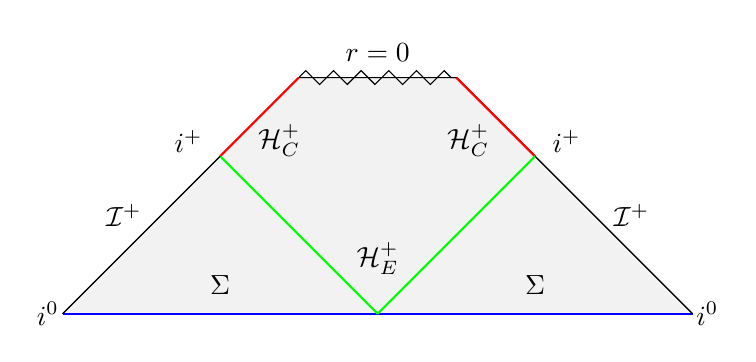
\begin{tikzpicture}
    \draw[fill=gray!10]    (-4,0) -- ++(3,3) -- ++ (2,0) --++ (3,-3);   
   \draw[decorate,decoration=zigzag]  (-1,3) -- (1,3)
    node[midway, above, inner sep=2mm] {$r=0$};
               \draw[red,thick] (2,2) -- (1,3);
                    \draw[red,thick] (-2,2) -- (-1,3);
                               \node[label=above:$\mathcal{H}_E^+$]  at (0,0.25) {};
                                    \draw[blue,thick] (-4,0) -- (4,0);
                                          \draw[green,thick] (-2,2) -- (0,0);
                                                \draw[green,thick] (2,2) -- (0,0);
                                                         \node[label=above:$\Sigma$]  at (-2,0) {};
                                                                  \node[label=above:$\Sigma$]  at (2,0) {};
                                    \draw (-2,2) -- (-4,0);{};  
                                       \draw (2,2) -- (4,0);{};    
            \node[label=above:$\mathcal{H}_C^+$]  at (-1.25,1.75) {};
               \node[label=above:$\mathcal{H}_C^+$]  at (1.15,1.75) {};
                      \node[label=right:$\mathcal{I}^+$]  at (2.75,1.25) {};
                                 \node[label=left:$\mathcal{I}^+$]  at (-2.75,1.25) {};    
                        \node[label=above:$i^+$]  at (2.4,1.8) {};
                          \node[label=above:$i^+$]  at (-2.4,1.8) {};
                                     \node[label=right:$i^0$]  at (3.8,0) {};
 \node[label=left:$i^0$]  at (-3.8,0) {};                                                   
    \end{tikzpicture}